% !TeX root = ../main.tex

%%% Tables %%%

\begin{table}[ht]
\centering
\caption{Estimates with standard errors for the parameters of the distributions of dive duration $(Y_t)$, acceleration $(\Zone_{t,\tilde t^*})$, and wiggliness $(\Ztwo_{t,\tilde t^*})$ of the killer whale kinematic data using the full CarHHMM-DFT. The parentheses refer to standard errors estimated using the observed information matrix.}
\scalebox{0.85}{
    \begin{tabular}{ccccc}
        \multirow{2}{*}{Feature}                                                       & \multirow{2}{*}{Dive / Subdive Type} & \multicolumn{3}{c}{Parameter Estimate}        \\
                                                                                       &                                      & $\hat \mu$    & $\hat \sigma$ & $\hat \phi$   \\ \hline
        \multirow{2}{*}{Dive Duration $(s)$ -- $Y_t$}                                  & 1                                    & $27.34 (0.63)$ & $10.96 (0.56)$ & ---           \\
                                                                                       & 2                                    & $127.5 (11.3)$ & $63.9 (9.0)$ & ---           \\ \hline
        \multirow{3}{*}{$x$-Acc. $(m/s^2)$ -- $\left(\Zone_{t,\tilde t^*}\right)_x$}   & 1                                    & $0.449 (0.030)$ & $0.039 (0.001)$ & $0.968 (0.002)$ \\
                                                                                       & 2                                    & $0.210 (0.012)$ & $0.096 (0.002)$ & $0.829 (0.007)$ \\
                                                                                       & 3                                    & $0.232 (0.035)$ & $0.296 (0.010)$ & $0.607 (0.023)$ \\ \hline
        \multirow{3}{*}{$y$-Acc. $(m/s^2)$ -- $\left(\Zone_{t,\tilde t^*}\right)_y$}   & 1                                    & $0.450 (0.038)$ & $0.051 (0.001)$ & $0.968 (0.002)$ \\
                                                                                       & 2                                    & $0.437 (0.012)$ & $0.094 (0.002)$ & $0.829 (0.007)$ \\
                                                                                       & 3                                    & $0.366 (0.042)$ & $0.365 (0.012)$ & $0.607 (0.023)$ \\ \hline
        \multirow{3}{*}{$z$-Acc. $(m/s^2)$ -- $\left(\Zone_{t,\tilde t^*}\right)_z$}   & 1                                    & $-0.691 (0.043)$ & $0.058 (0.001)$ & $0.968 (0.002)$ \\
                                                                                       & 2                                    & $-0.573 (0.014)$ & $0.111 (0.002)$ & $0.829 (0.007)$ \\
                                                                                       & 3                                    & $-0.303 (0.041)$ & $0.354 (0.012)$ & $0.607 (0.023)$ \\ \hline
        \multirow{3}{*}{Wiggliness - $\Ztwo_{t,\tilde t^*}$}                           & 1                                    & $34.02 (0.36)$ & $22.99 (0.38)$ & ---           \\
                                                                                       & 2                                    & $490.1 (5.6)$ & $502.6 (6.8)$ & ---           \\
                                                                                       & 3                                    & $9150 (220)$ & $13540 (350)$ & ---           \\ \hline
    \end{tabular}
    }
    \label{table:emis_dists_CarHHMM-DFT}
\end{table}

\begin{table}[ht]
\centering
\caption{Average decoding accuracies and training times for all models in the simulation study. Each of the four models was fit to 500 training data sets comprised of 100 simulated dives and tested on test data sets also comprised of 100 simulated dives. Reported values are averages, and $\pm$ refers to the sample standard deviation across the 500 data sets. Rows labelled Both/Both correspond to overall average decoding accuracy.}
\scalebox{0.5}{
\begin{tabular}{ccccccc}
Model                       & \multicolumn{1}{c}{Train Time (m)} & \multicolumn{1}{c}{Dive Type} & \multicolumn{1}{c}{Subdive Type} & \multicolumn{1}{c}{Dive Accuracy} & \multicolumn{1}{c}{Subdive Accuracy}  \\ \hline
\multirow{7}{*}{CarHHMM-DFT}& \multirow{7}{*}{$156 \pm 67$}   & All                           & All                              & $0.956 \pm 0.028$                   & $0.911 \pm 0.006$                       \\
                            &                                    & 1                             & 1                                & \multirow{3}{*}{$0.973\pm0.032$}    & $0.846 \pm 0.027$                       \\
                            &                                    & 1                             & 2                                &                                   & $0.918 \pm 0.011$                       \\ 
                            &                                    & 1                             & 3                                &                                   & $0.860 \pm 0.030$                       \\ 
                            &                                    & 2                             & 1                                & \multirow{3}{*}{$0.856\pm0.097$}    & $0.949 \pm 0.010$                       \\ 
                            &                                    & 2                             & 2                                &                                   & $0.915 \pm 0.015$                       \\
                            &                                    & 2                             & 3                                &                                   & $0.871 \pm 0.057$                       \\ \hline
\multirow{7}{*}{HHMM-DFT}   & \multirow{7}{*}{$162 \pm 64$}   & All                           & All                              & $0.959 \pm 0.025$                   & $0.844 \pm 0.024$                       \\
                            &                                    & 1                             & 1                                & \multirow{3}{*}{$0.977\pm0.028$}    & $0.761 \pm 0.063$                       \\ 
                            &                                    & 1                             & 2                                &                                   & $0.845 \pm 0.029$                       \\ 
                            &                                    & 1                             & 3                                &                                   & $0.858 \pm 0.034$                       \\
                            &                                    & 2                             & 1                                & \multirow{3}{*}{$0.851\pm0.097$}    & $0.883 \pm 0.066$                       \\ 
                            &                                    & 2                             & 2                                &                                   & $0.829 \pm 0.041$                       \\
                            &                                    & 2                             & 3                                &                                   & $0.876 \pm 0.061$                       \\ \hline
\multirow{7}{*}{CarHHMM}    & \multirow{7}{*}{$258 \pm 106$}   & All                           & All                              & $0.924 \pm 0.127$                   & $0.845 \pm 0.018$                       \\
                            &                                    & 1                             & 1                                & \multirow{3}{*}{$0.933\pm0.153$}    & $0.689 \pm 0.050$                       \\ 
                            &                                    & 1                             & 2                                &                                   & $0.900 \pm 0.031$                       \\ 
                            &                                    & 1                             & 3                                &                                   & $0.673 \pm 0.059$                       \\
                            &                                    & 2                             & 1                                & \multirow{3}{*}{$0.864\pm0.134$}    & $0.906 \pm 0.022$                       \\ 
                            &                                    & 2                             & 2                                &                                   & $0.848 \pm 0.033$                       \\
                            &                                    & 2                             & 3                                &                                   & $0.687 \pm 0.105$                       \\ \hline
\multirow{7}{*}{CarHMM-DFT} & \multirow{7}{*}{$45 \pm 22$}   & All                           & All                              & ---                                   & $0.912 \pm 0.006$                       \\
                            &                                    & 1                             & 1                                & \multirow{3}{*}{---          }    & $0.854 \pm 0.026$                       \\
                            &                                    & 1                             & 2                                &                                   & $0.921 \pm 0.011$                       \\                            
                            &                                    & 1                             & 3                                &                                   & $0.860 \pm 0.032$                       \\ 
                            &                                    & 2                             & 1                                & \multirow{3}{*}{---          }    & $0.943 \pm 0.011$                       \\ 
                            &                                    & 2                             & 2                                &                                   & $0.919 \pm 0.014$                       \\ 
                            &                                    & 2                             & 3                                &                                   & $0.878 \pm 0.053$                       \\ \hline
\end{tabular}
}

\label{table:accuracy}
\end{table}

%%% model definitions %%%

\begin{figure}[ht]
    \begin{subfigure}{\textwidth}
      \centering
      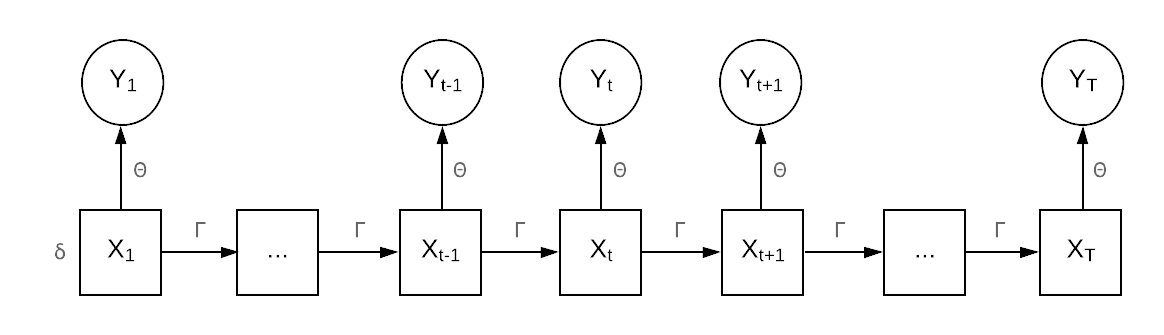
\includegraphics[width=3.5in]{../Plots/HMM.png}  
      \label{fig:HMM}
    \end{subfigure}
    %
    \hrule
    %
    \begin{subfigure}{\textwidth}
      \centering
      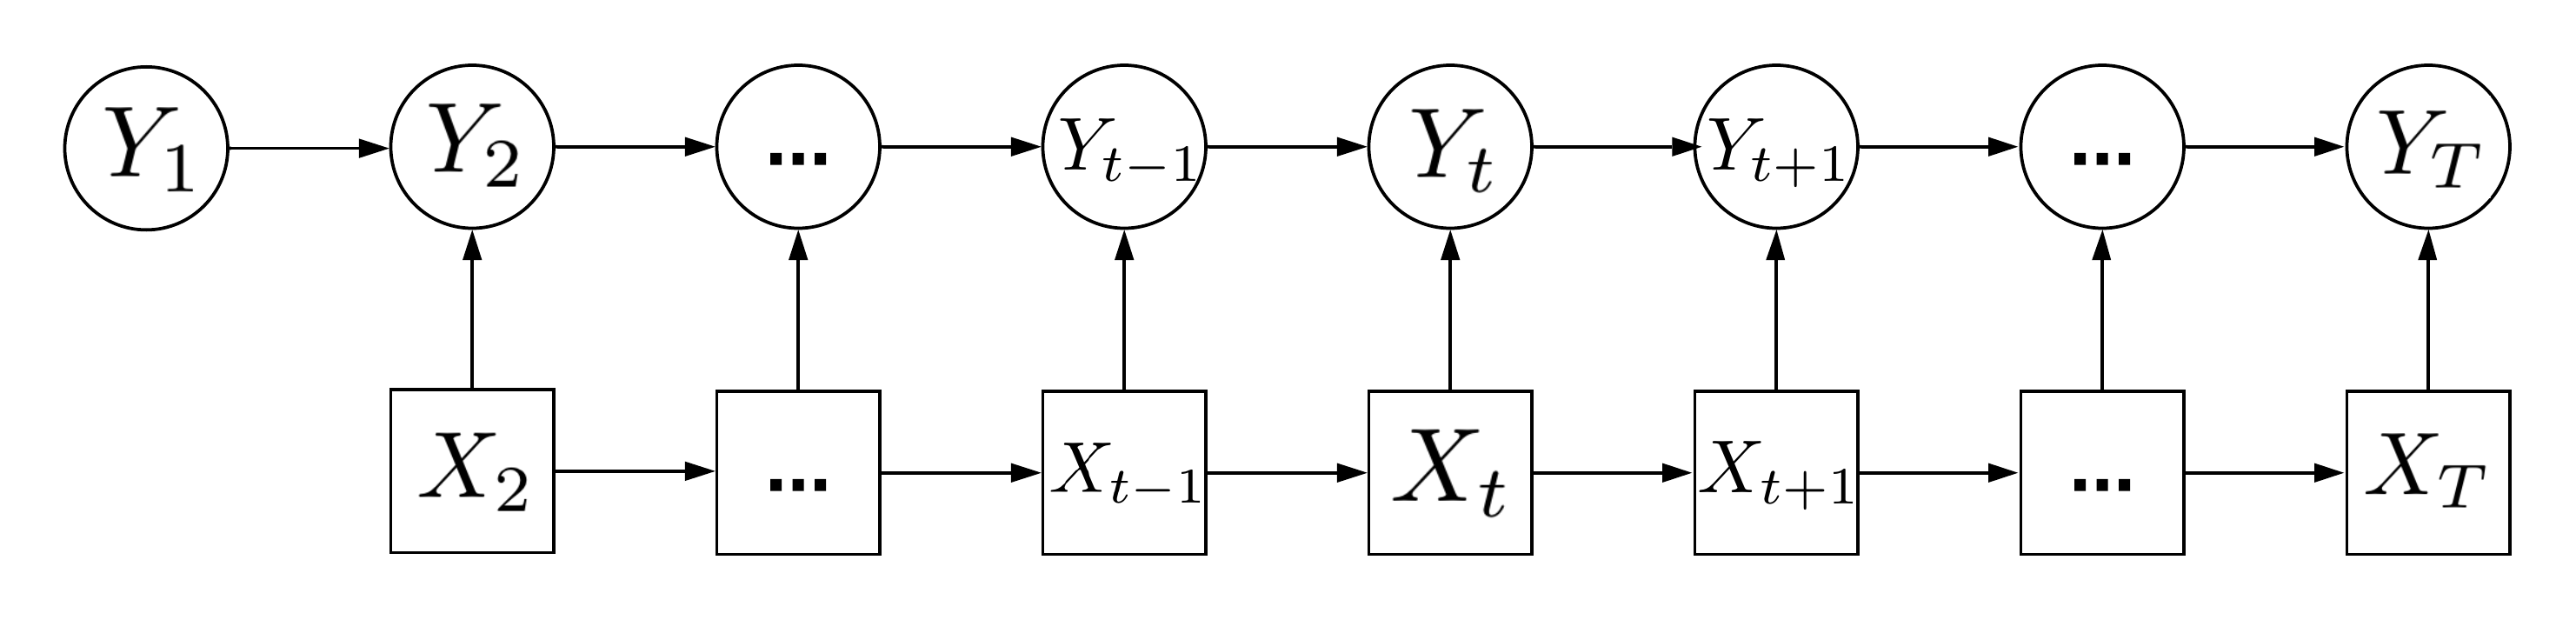
\includegraphics[width=3.5in]{../Plots/CarHMM.png}  
      \label{fig:CarHMM}
    \end{subfigure}
    %
    \hrule
    %
    \begin{subfigure}{\textwidth}
      \centering
      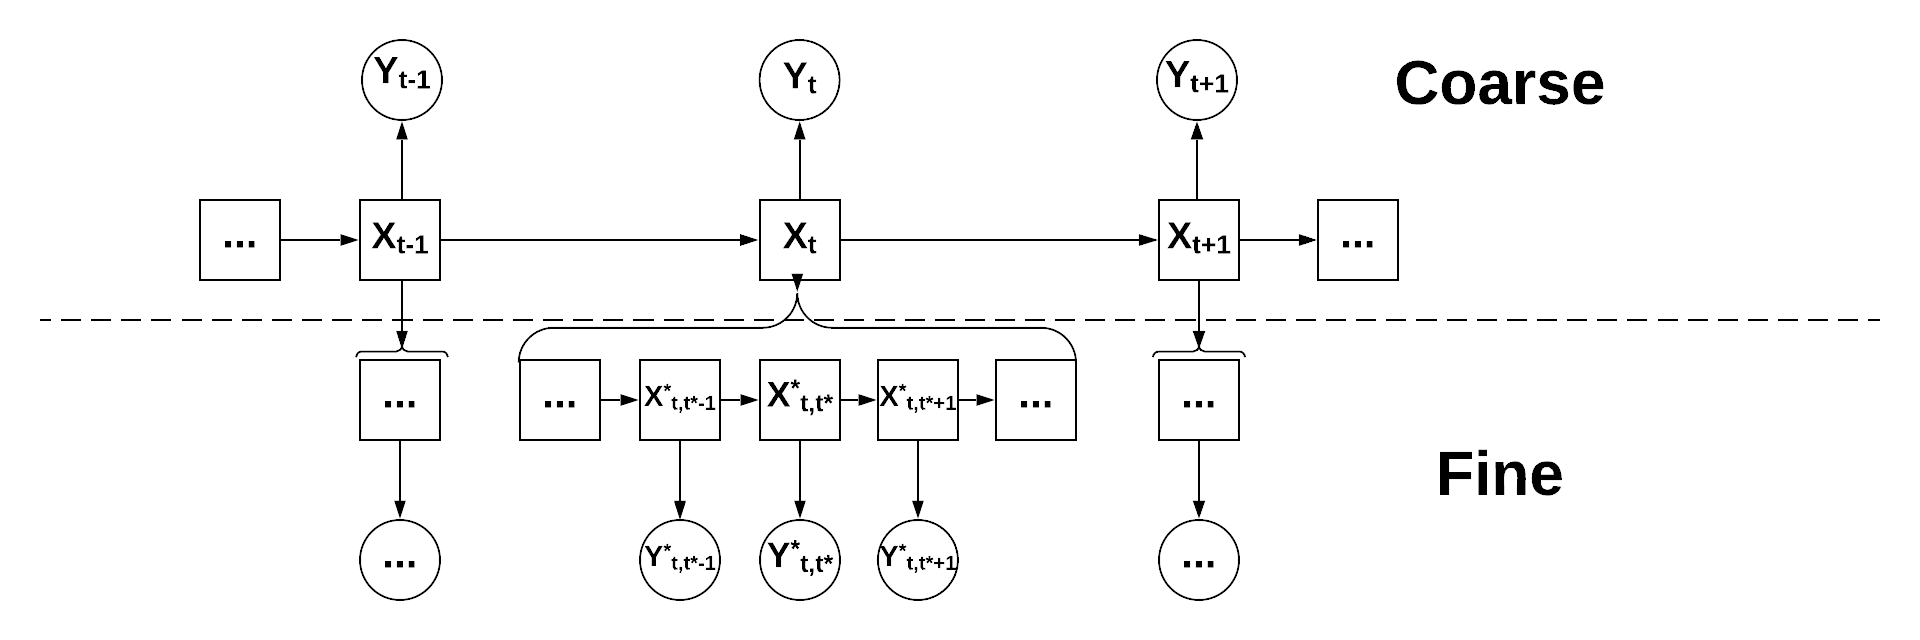
\includegraphics[width=3.75in]{../Plots/HHMM.png}  
      \label{fig:HHMM}
    \end{subfigure}
    %
    \hrule
    %
    \begin{subfigure}{\textwidth}
      \centering
      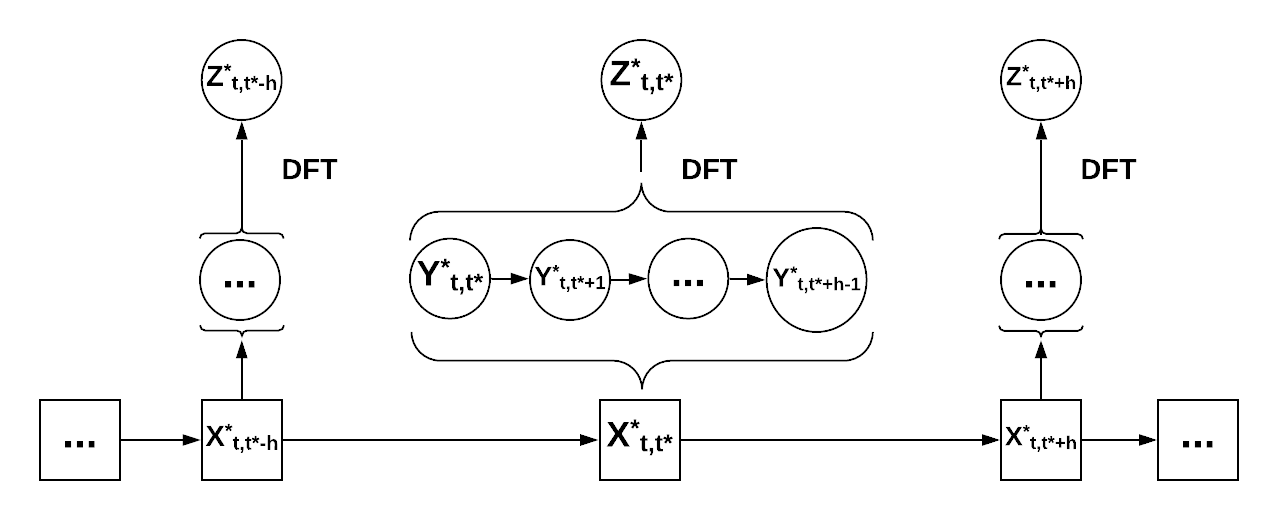
\includegraphics[width=3.5in]{../Plots/HMM-DFT.png}  
      \label{fig:HMM-DFT}
    \end{subfigure}
    \caption{Dependence structure of a standard HMM (top), CarHMM (middle-top), HHMM (middle-bottom), and HMM-DFT (bottom). Hidden state sequences are denoted as $X$ on the coarse-scale and $X^*$ on the fine scale. Observations are denoted as $Y$ on the coarse scale and $Y^*$ on the fine scale. The coarse-scale process is not included in the HMM-DFT because moving window transformations often only apply to fine-scale data. The fine-scale observations of the HMM-DFT are transformed using a moving window and denoted as $\Z$ with corresponding fine-scale hidden states $\tilde X^*$.}
    \label{fig:models}
\end{figure}

%%% data %%%

\begin{figure}[ht]
	\centering
	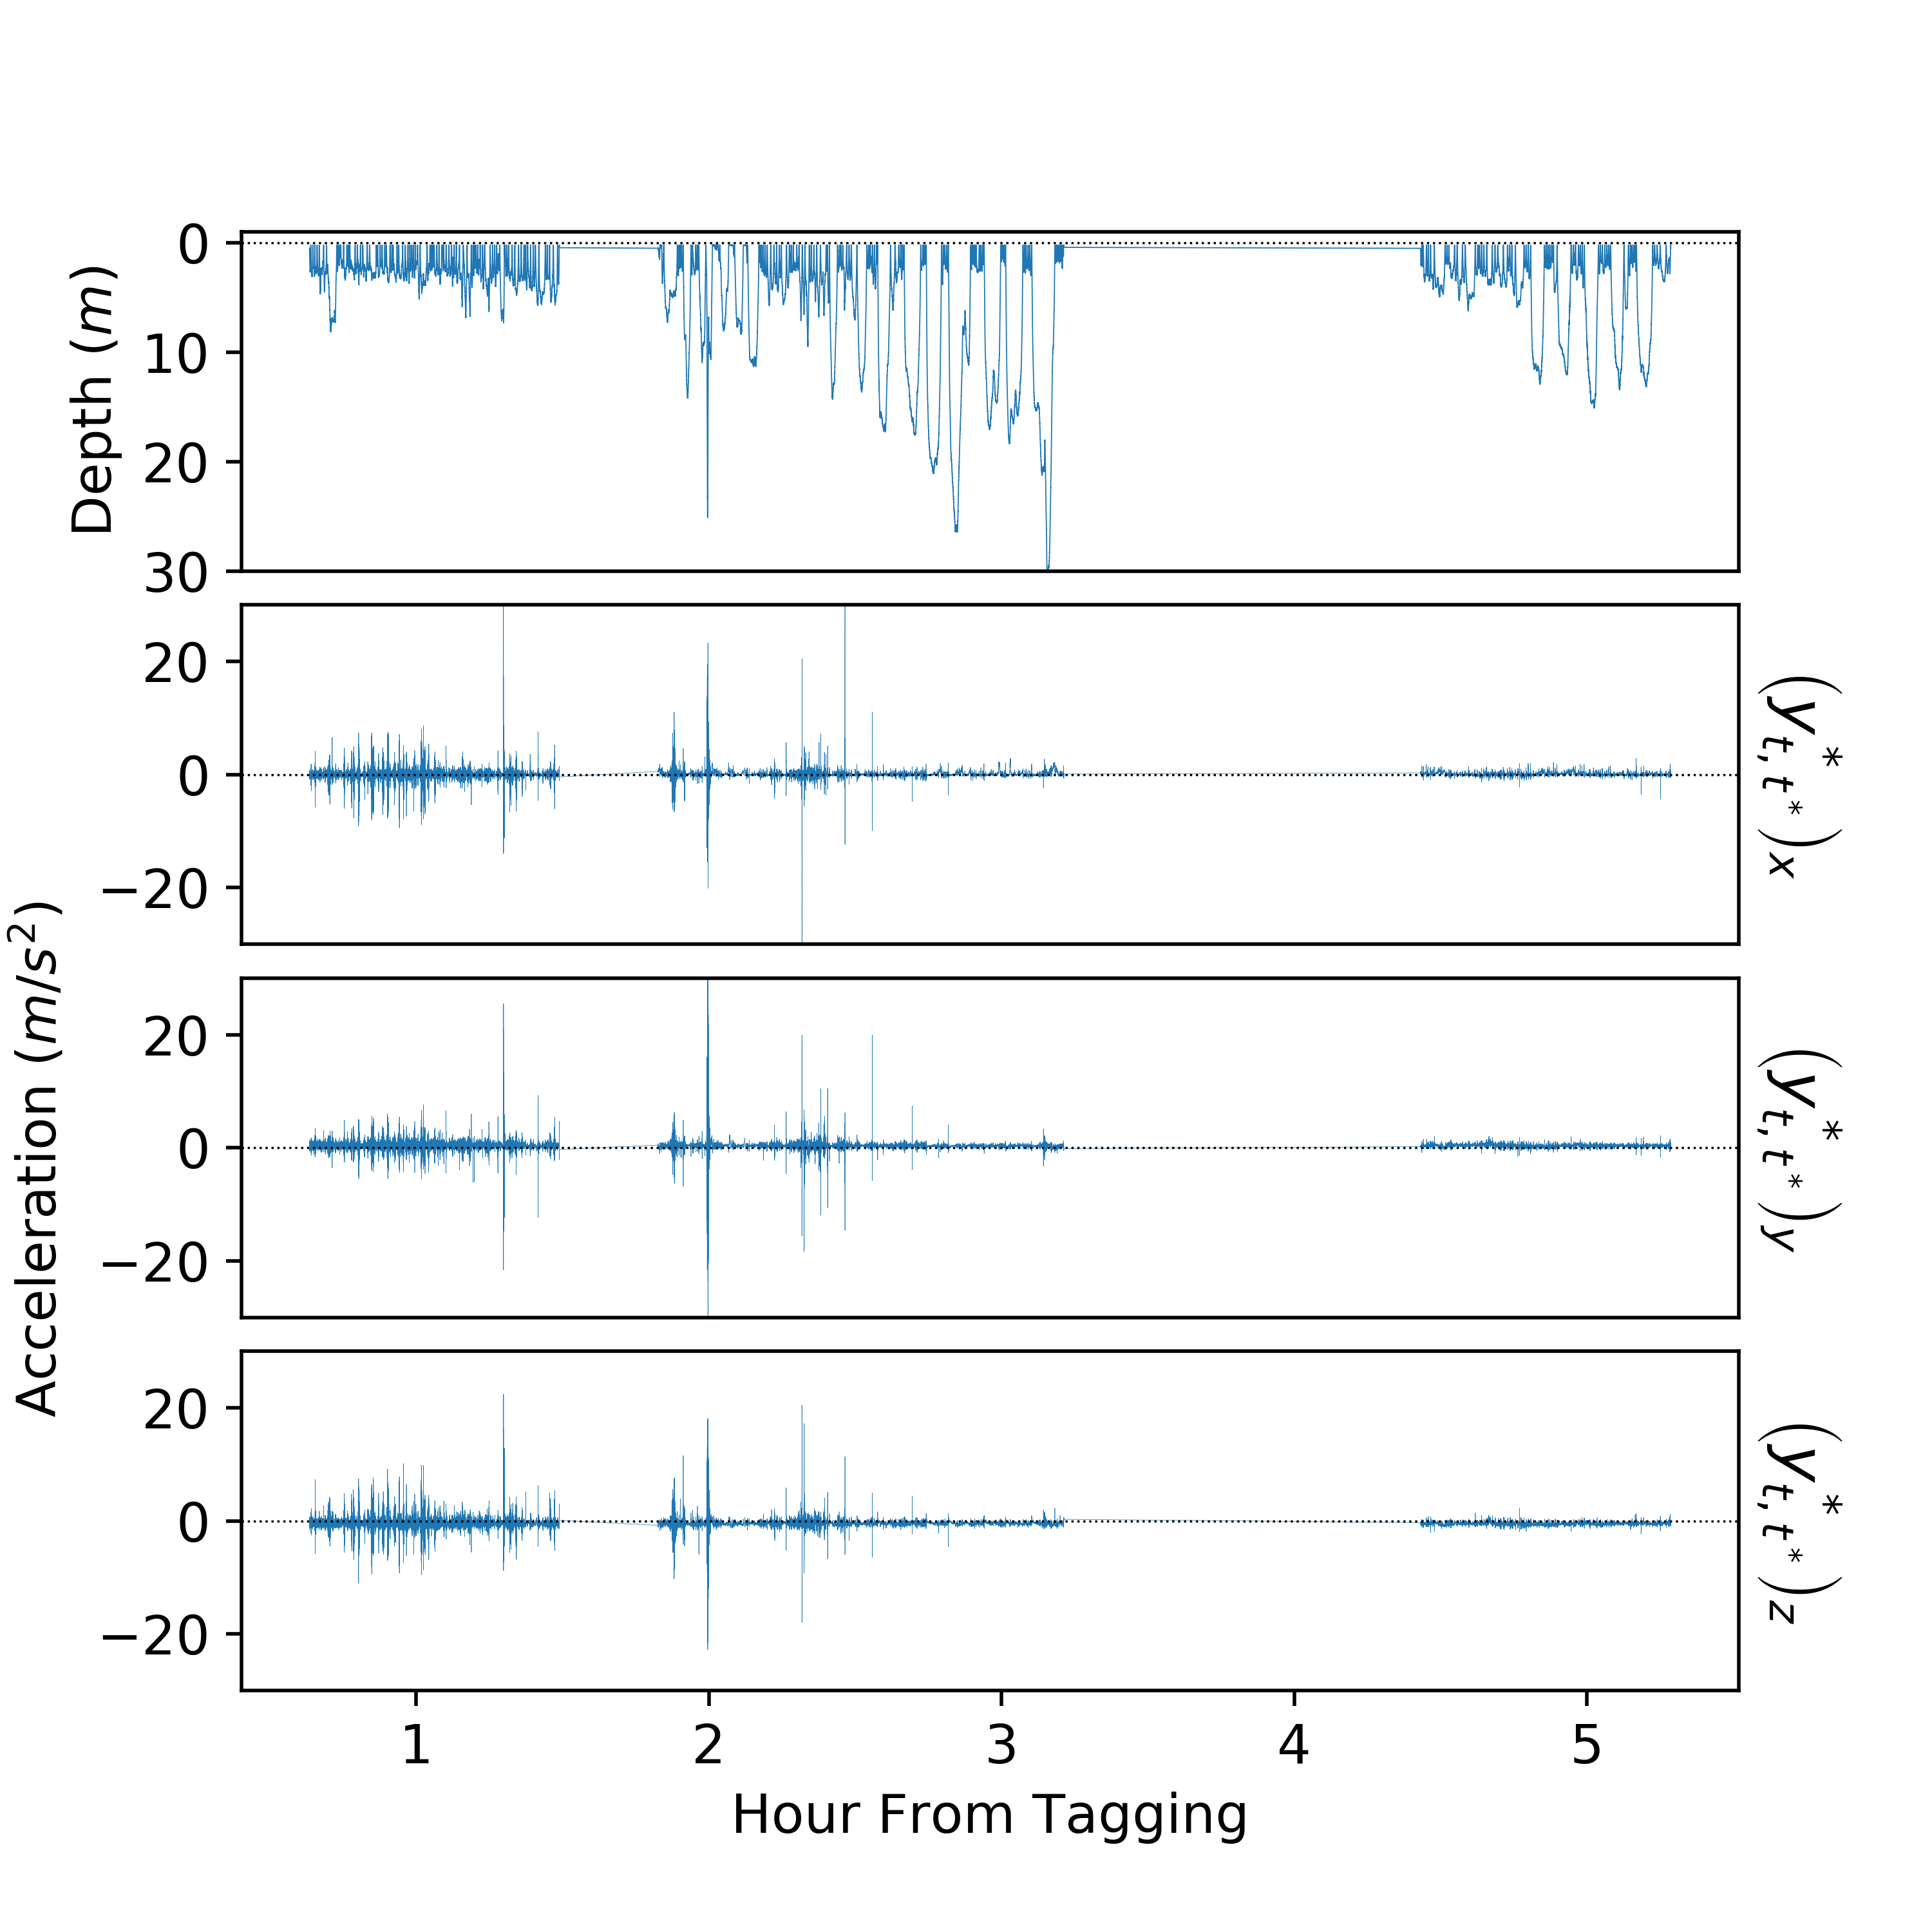
\includegraphics[width=5.25in]{../Plots/raw_data.png}
	\caption{Dive depth (top panel) and three-dimensional acceleration (bottom three panels) from a killer whale over approximately 5 hours. An exact physical interpretation of each of component acceleration is difficult due to variations in tag orientation. There are data gaps occurring from around $1.5$ to $1.8$ hours and from around $3.2$ to $4.5$ hours. Both data gaps were excluded from analyses.}
	\label{fig:data}
\end{figure}

%%% Case Study %%%

\begin{figure}[ht]
	\centering
	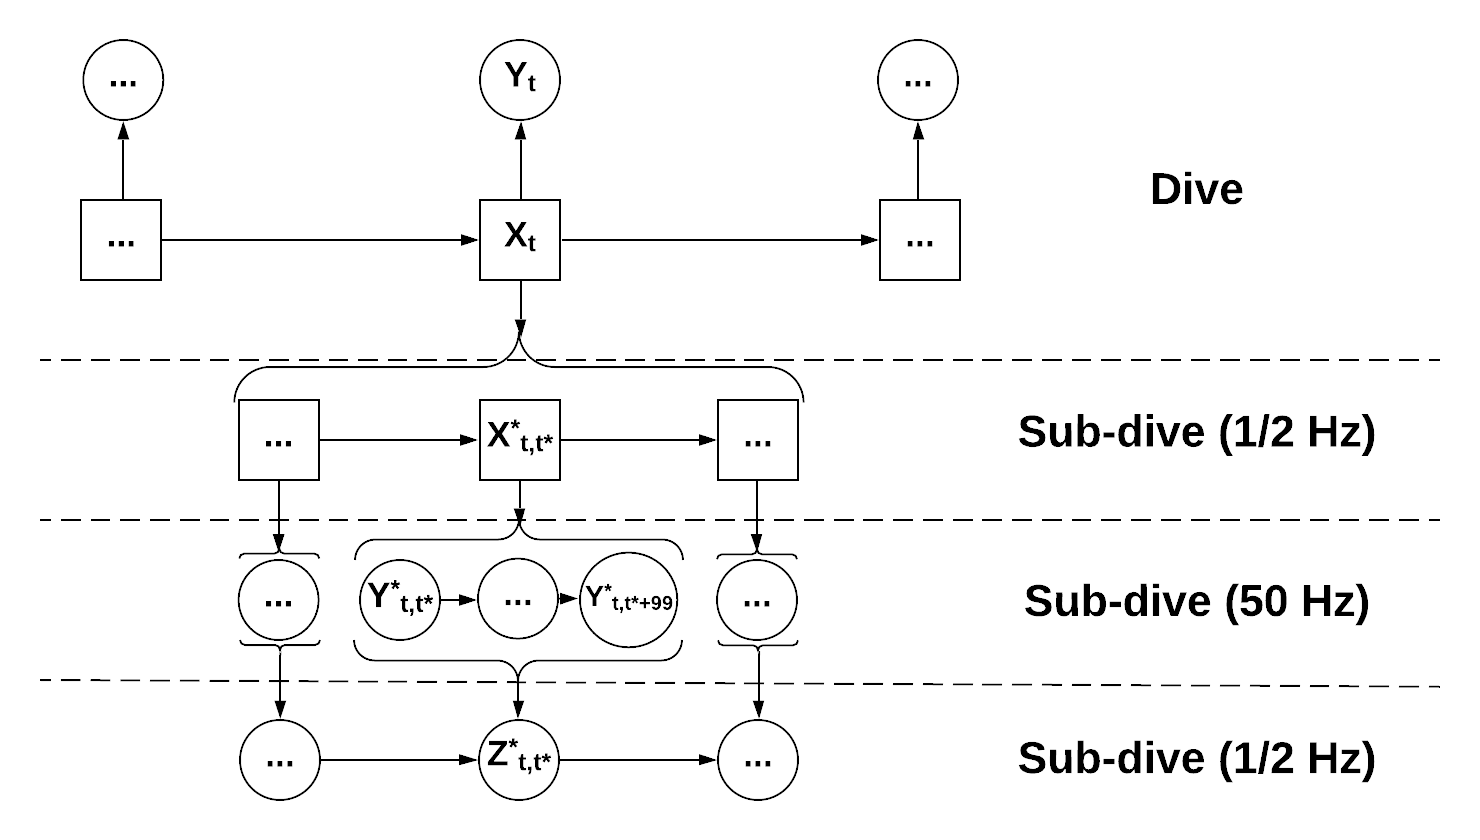
\includegraphics[width=5in]{../Plots/CarHHMM-DFT.png}
	\caption{Graphical representation of the conditionally auto-regressive hierarchical hidden Markov model with discrete Fourier transform (\textbf{CarHHMM-DFT}) used in the simulation and case study. The type of dive $t$ is denoted by $X_t$ and $Y_t$ represents the associated dive duration. The raw acceleration vector associated with dive $t$ and time stamp $t^*$ is denoted by $Y^*_{t,t^*}$. The subdive state of the killer whale during dive $t$ and window $\tilde t^*$ is denoted as $\tilde X^*_{t,\tilde t^*}$, and the corresponding transformed observation is denoted by $\Z_{t,\tilde t^*}$.}
	\label{fig:CarHHMM-DFT}
\end{figure}

\begin{figure}[ht]
    \begin{subfigure}{\textwidth}
    	\centering
    	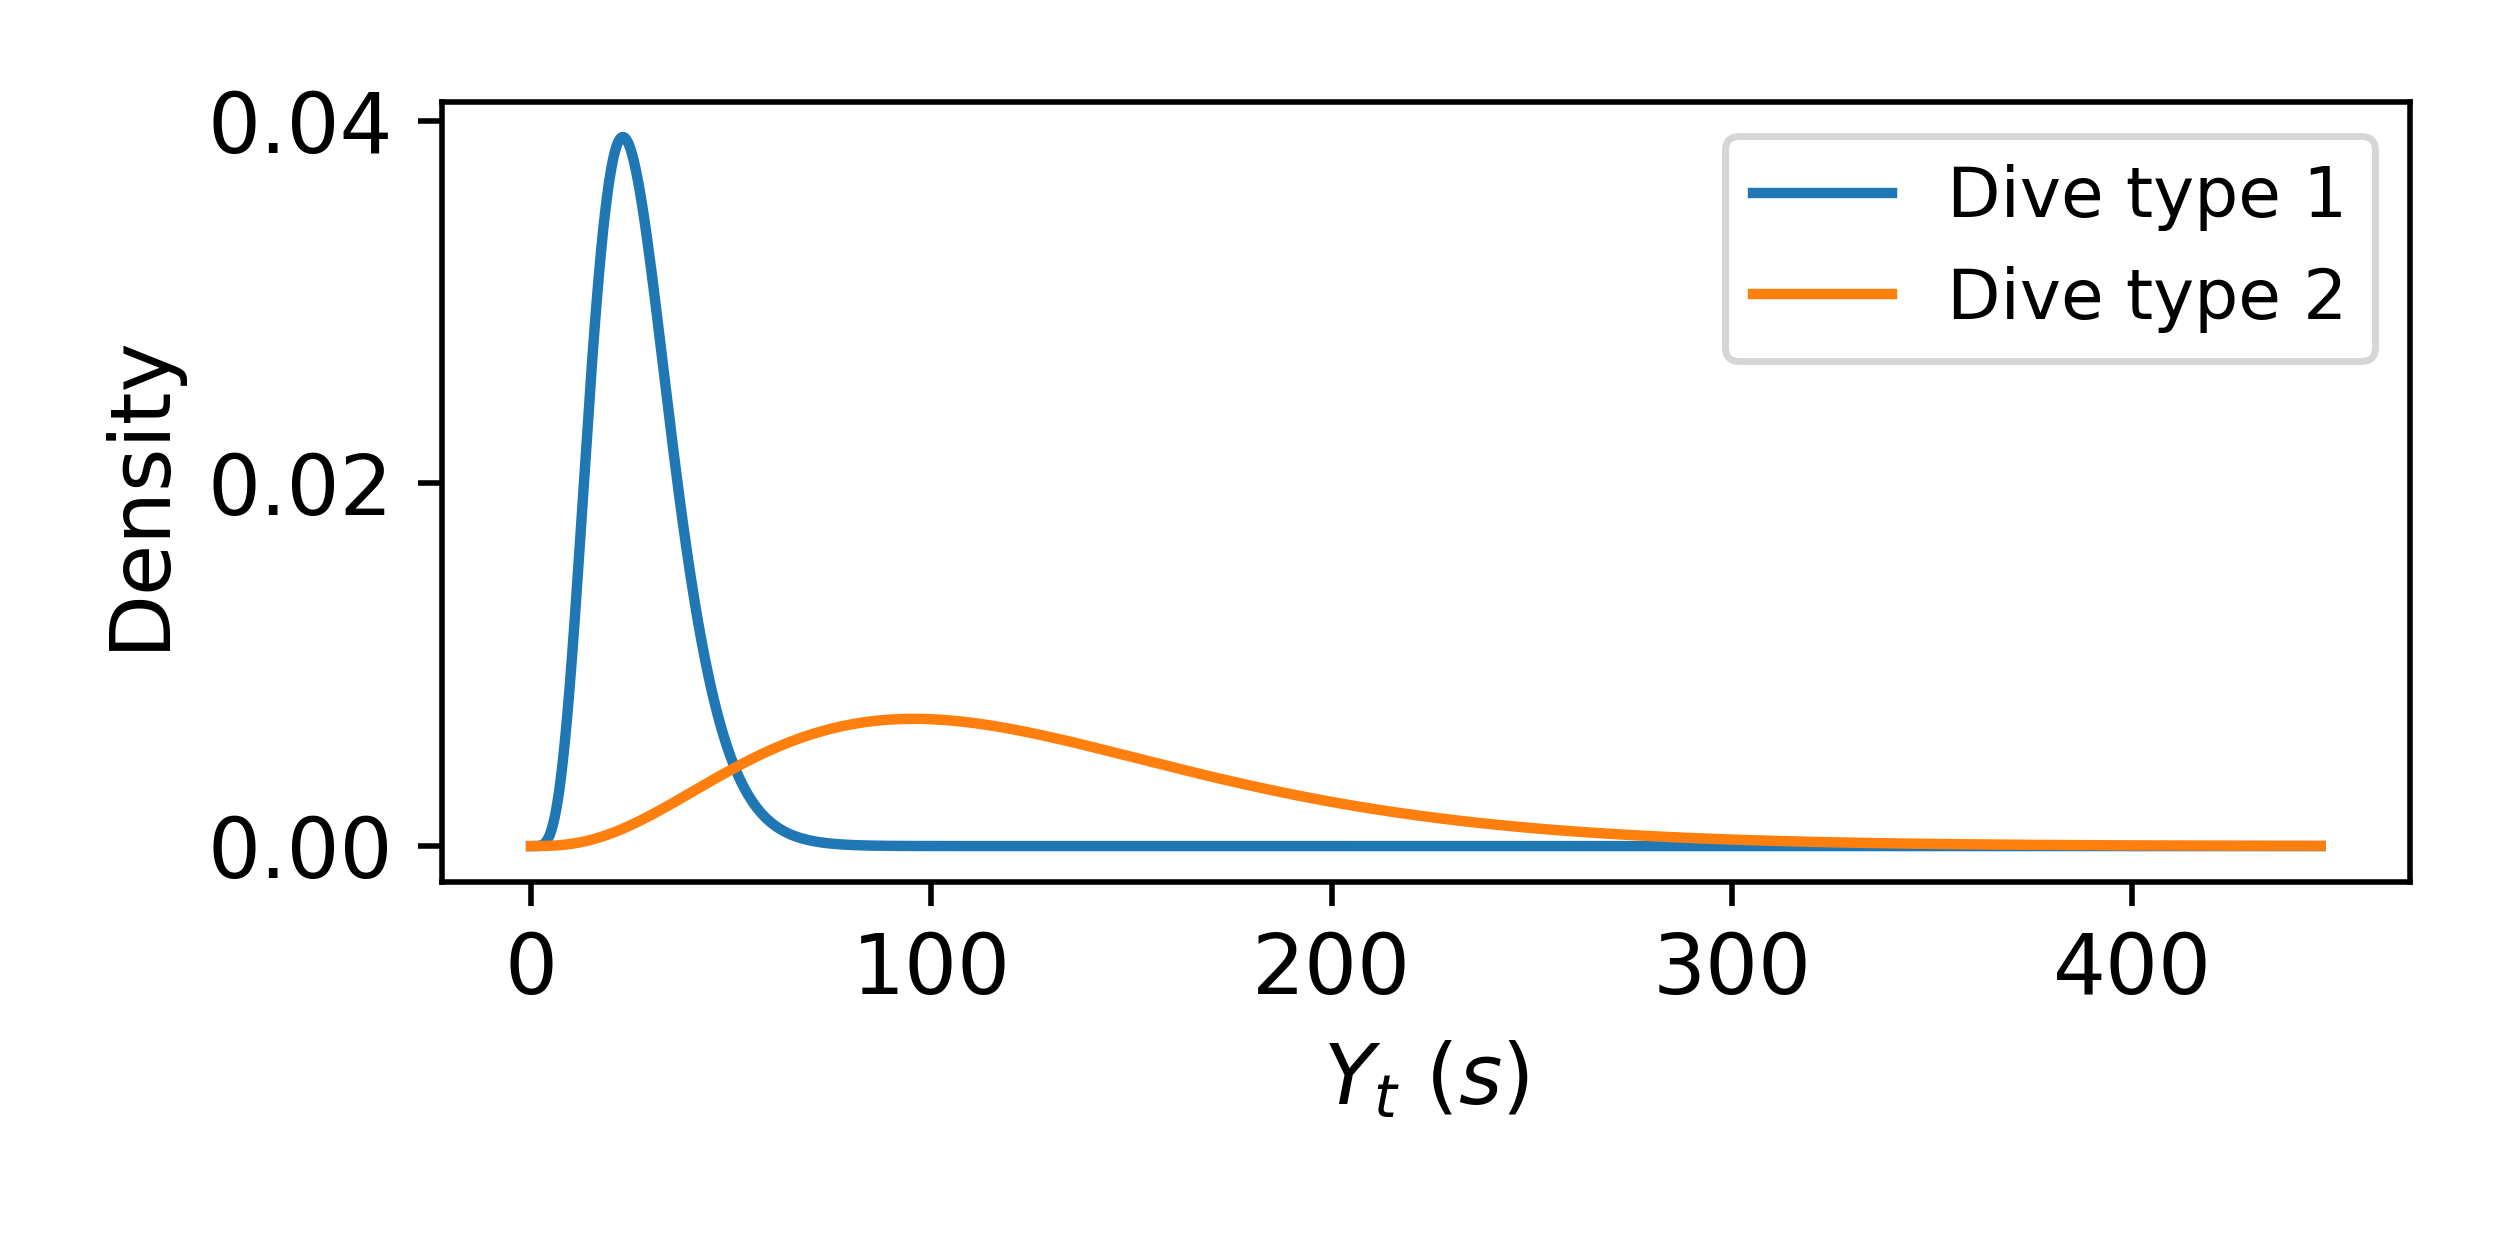
\includegraphics[width=3.25in]{../Plots/2019/20190902-182840-CATs_OB_1_0_267_CarHHMM2-coarse-emissions.png}
    \end{subfigure}
    \newline
    \begin{subfigure}{\textwidth}
    	\centering
    	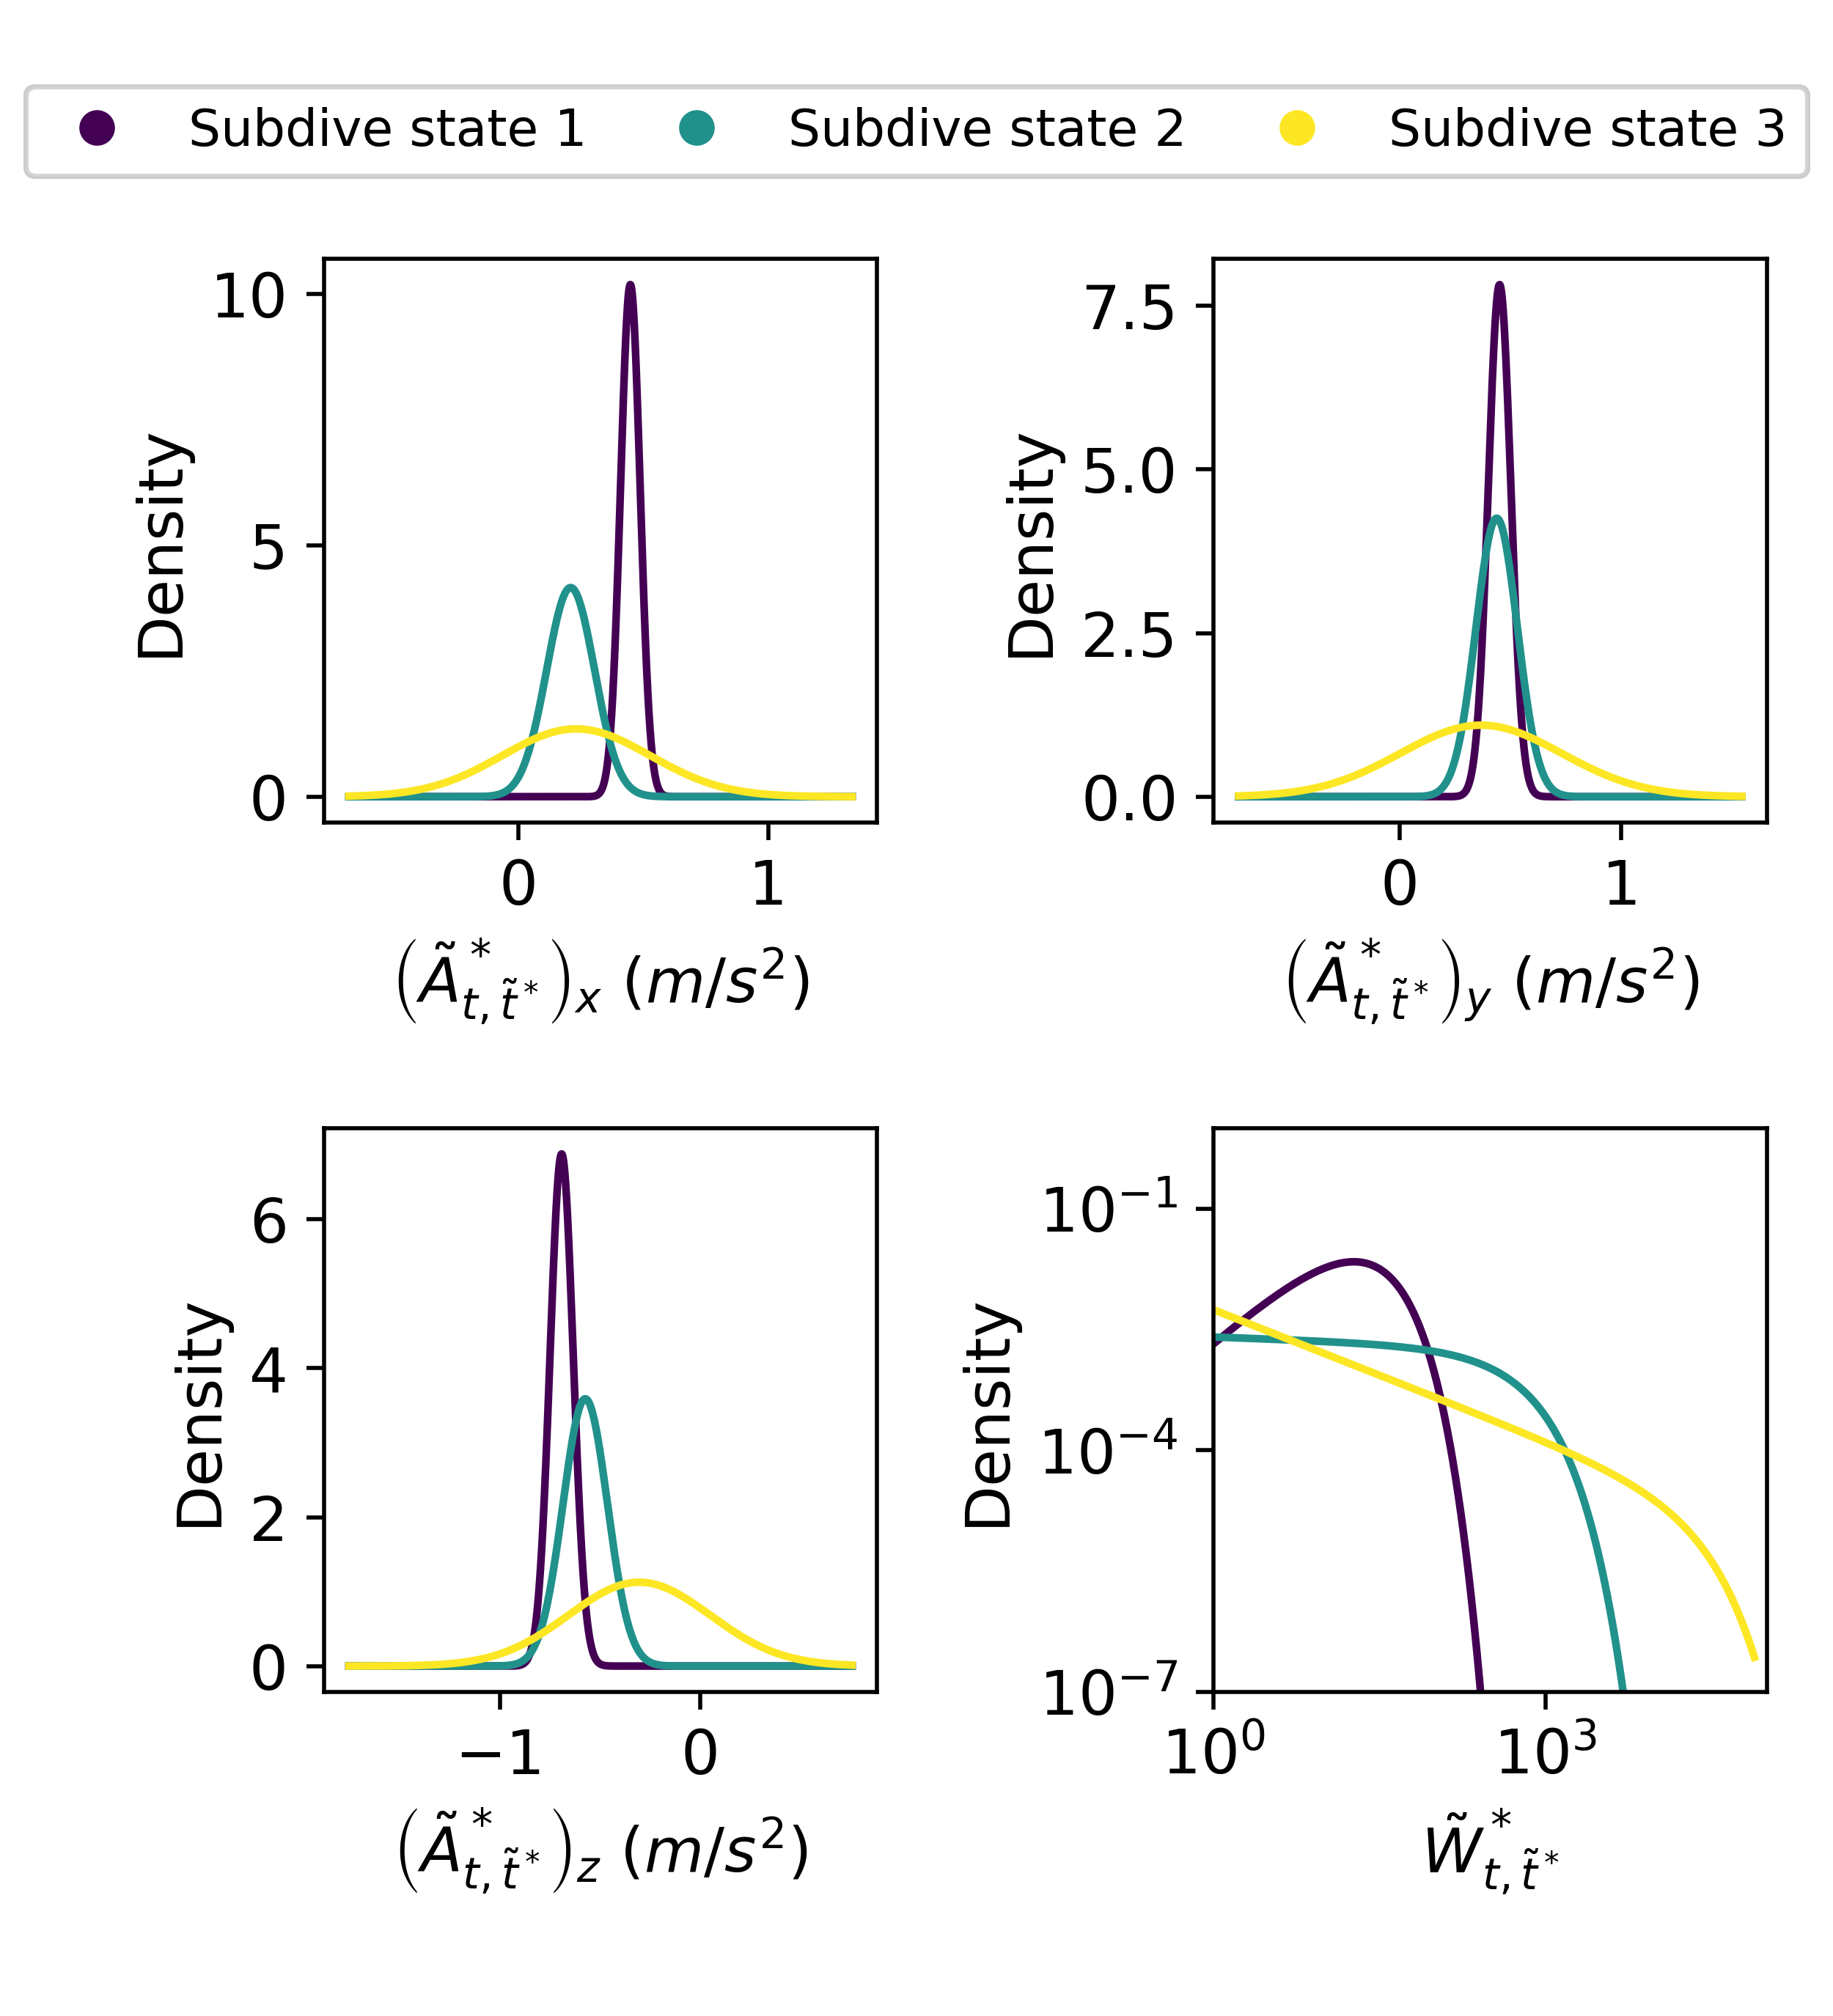
\includegraphics[width=3.25in]{../Plots/2019/20190902-182840-CATs_OB_1_0_267_CarHHMM2-fine-emissions.png}
    \end{subfigure}
    \caption{Estimated Gamma densities of killer whale dive duration ($Y_t$) (top), estimated Normal conditional densities of killer whale acceleration $(\Zone_{t,\tilde t^*}\big|\Zone_{t,\tilde t^*-1} = \mu_A^{*(\cdot,i^*)})$ (middle and bottom left), and estimated Gamma densities of wiggliness $(\Ztwo_{t,\tilde t^*})$ plotted on a log-log scale (bottom right). Densities of $Y_t$ correspond to dive types 1 and 2, while densities of $\Zone_{t,\tilde t^*}$ and $\Ztwo_{t,\tilde t^*}$ correspond to subdive states 1, 2, and 3. Densities are estimated by fitting the CarHHMM-DFT to the case study data (see Table \ref{table:emis_dists_CarHHMM-DFT}).}
    \label{fig:emis}
\end{figure}

\begin{figure}[ht]
	\centering
	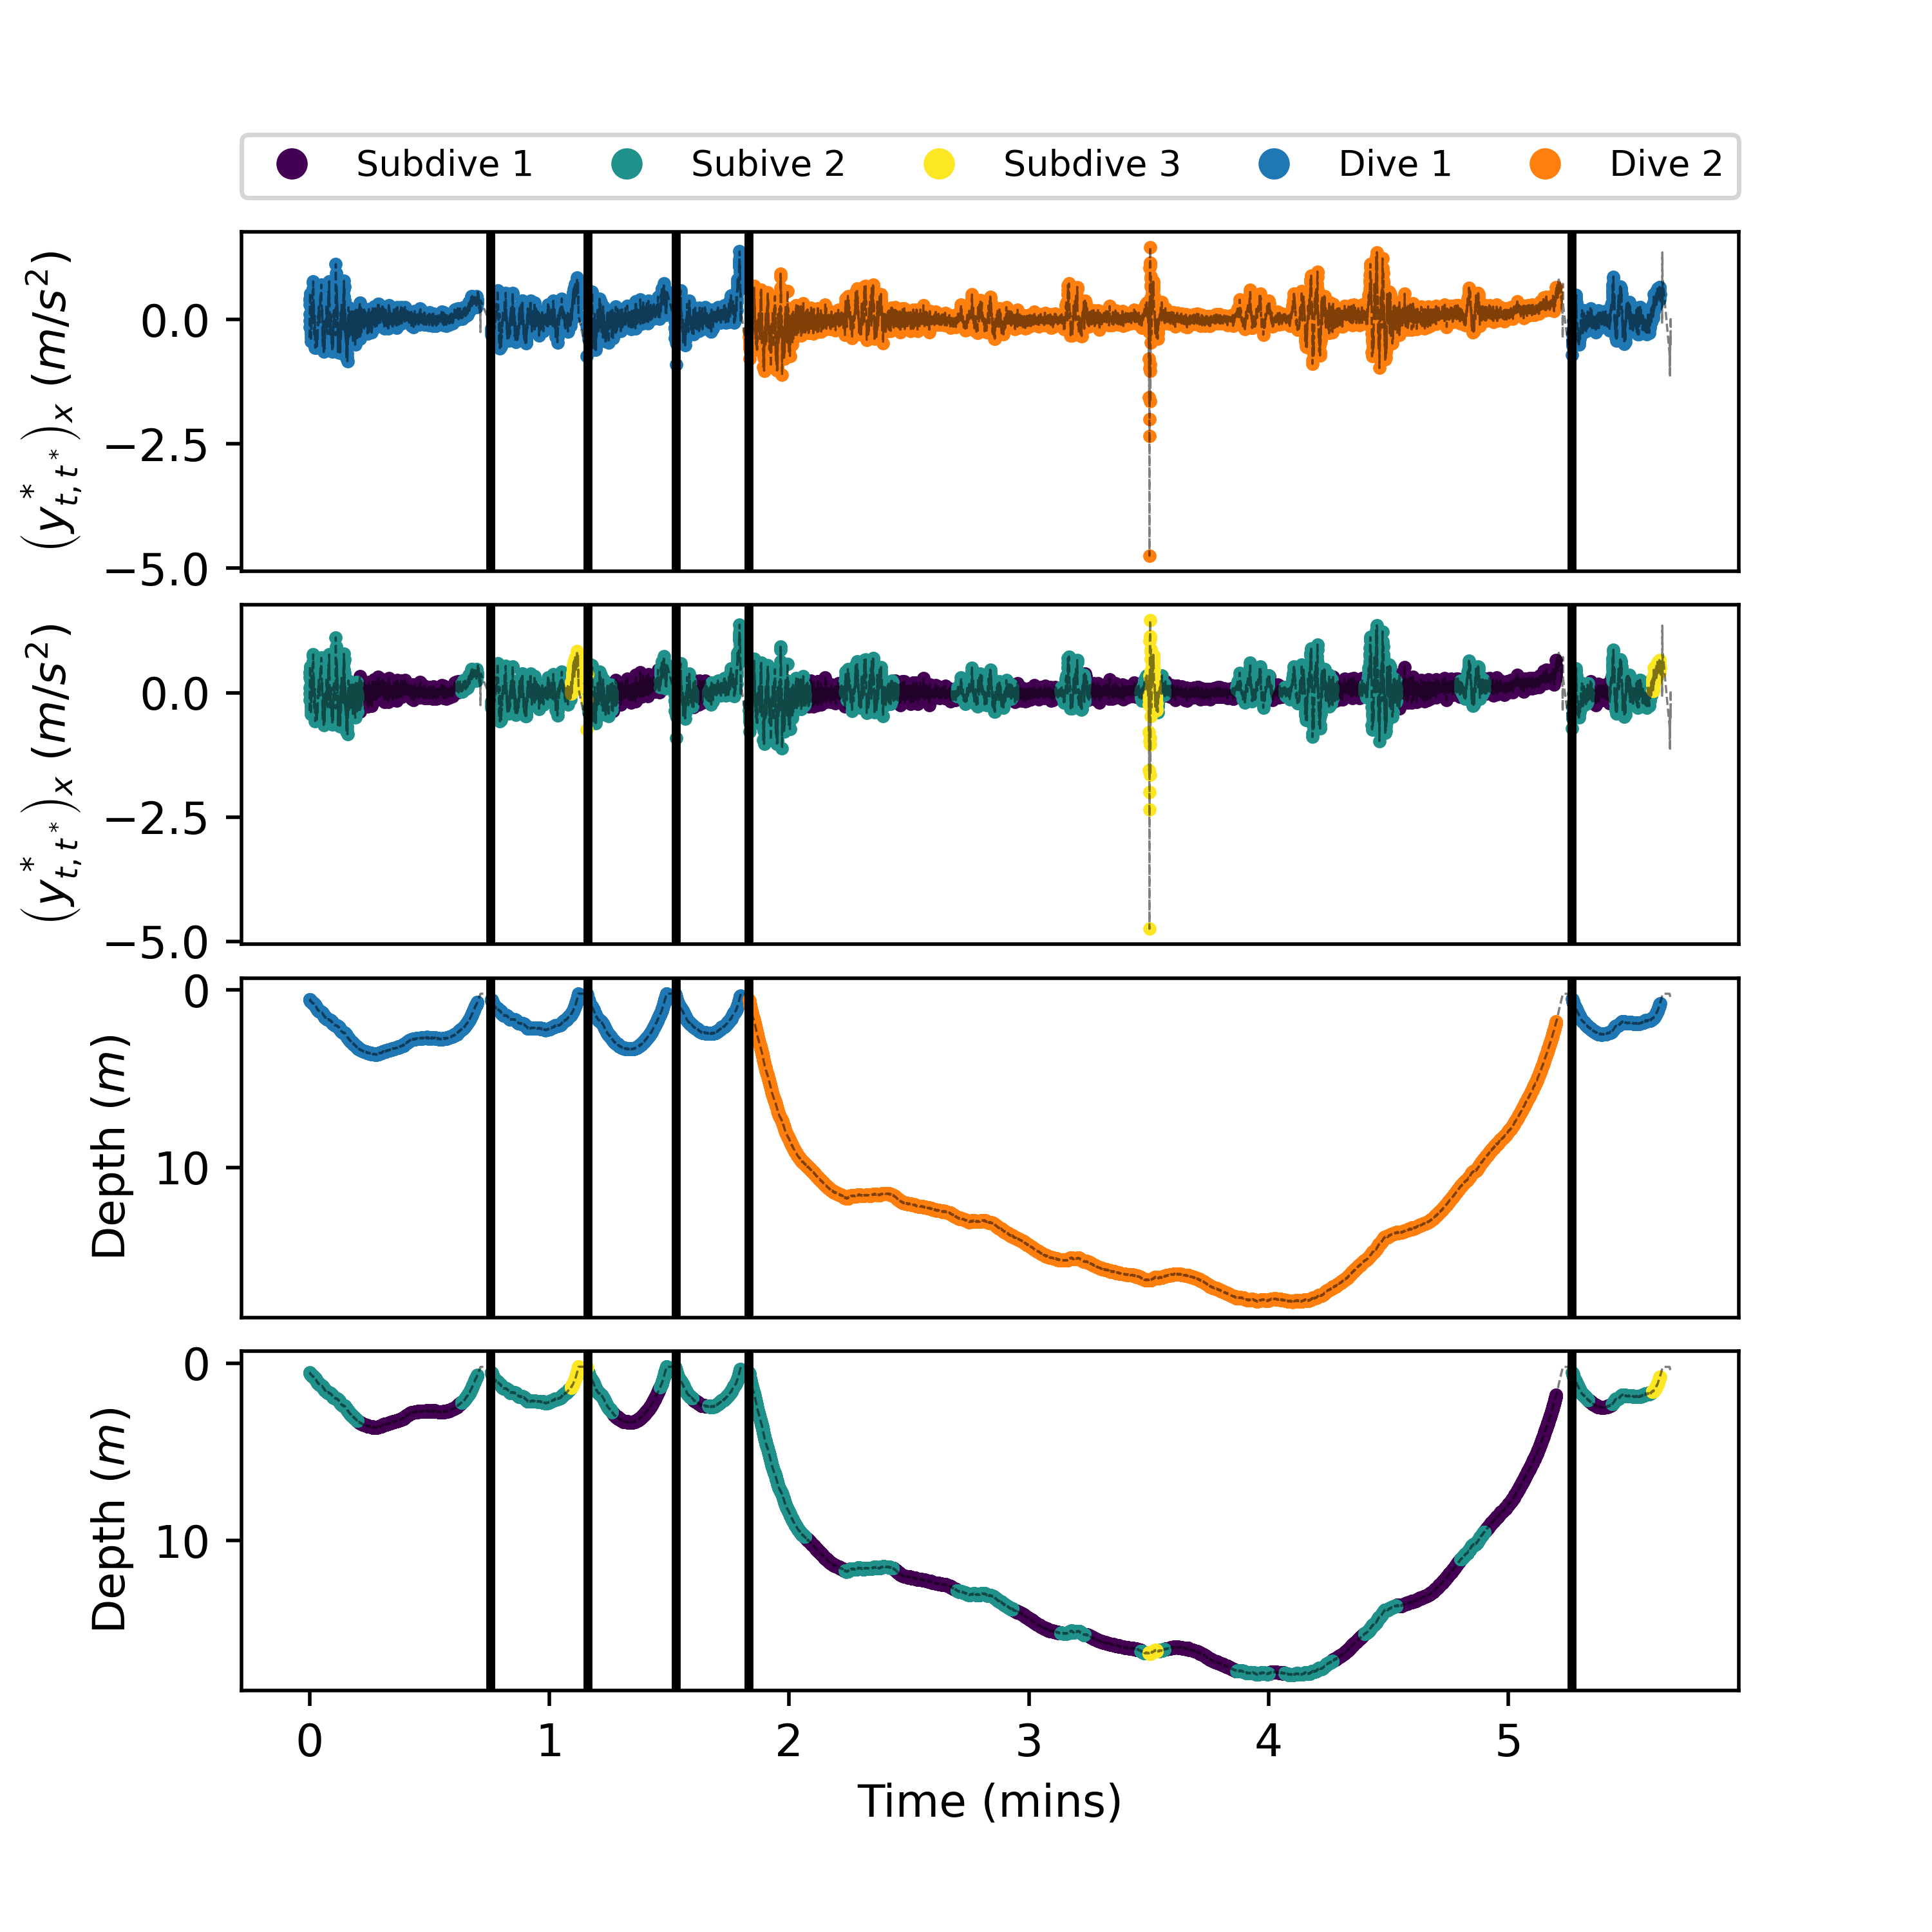
\includegraphics[width=4.75in]{../Plots/2019/20190902-182840-CATs_OB_1_0_267_CarHHMM2_decoded_dives.png}
	\caption{The $x$- component of acceleration $(y^*_{t,t^*})_x$ (top two panels) and dive depth (bottom two panels) of a northern resident killer whale for a sequence of six selected dives. Each panel is partitioned into dives by vertical black lines. The curve colours in the first and third panels correspond to the estimated dive types while the curve colours of the second and fourth panels correspond the estimated subdive states. Both the dive types and subdive states are estimated by fitting the CarHHMM-DFT to the data and performing the forward-backward algorithm to determine the hidden state with the highest probability.}
	\label{fig:labeled_dives}
\end{figure}

\begin{figure}[ht]
    \begin{subfigure}{0.45\textwidth}
    	\centering
    	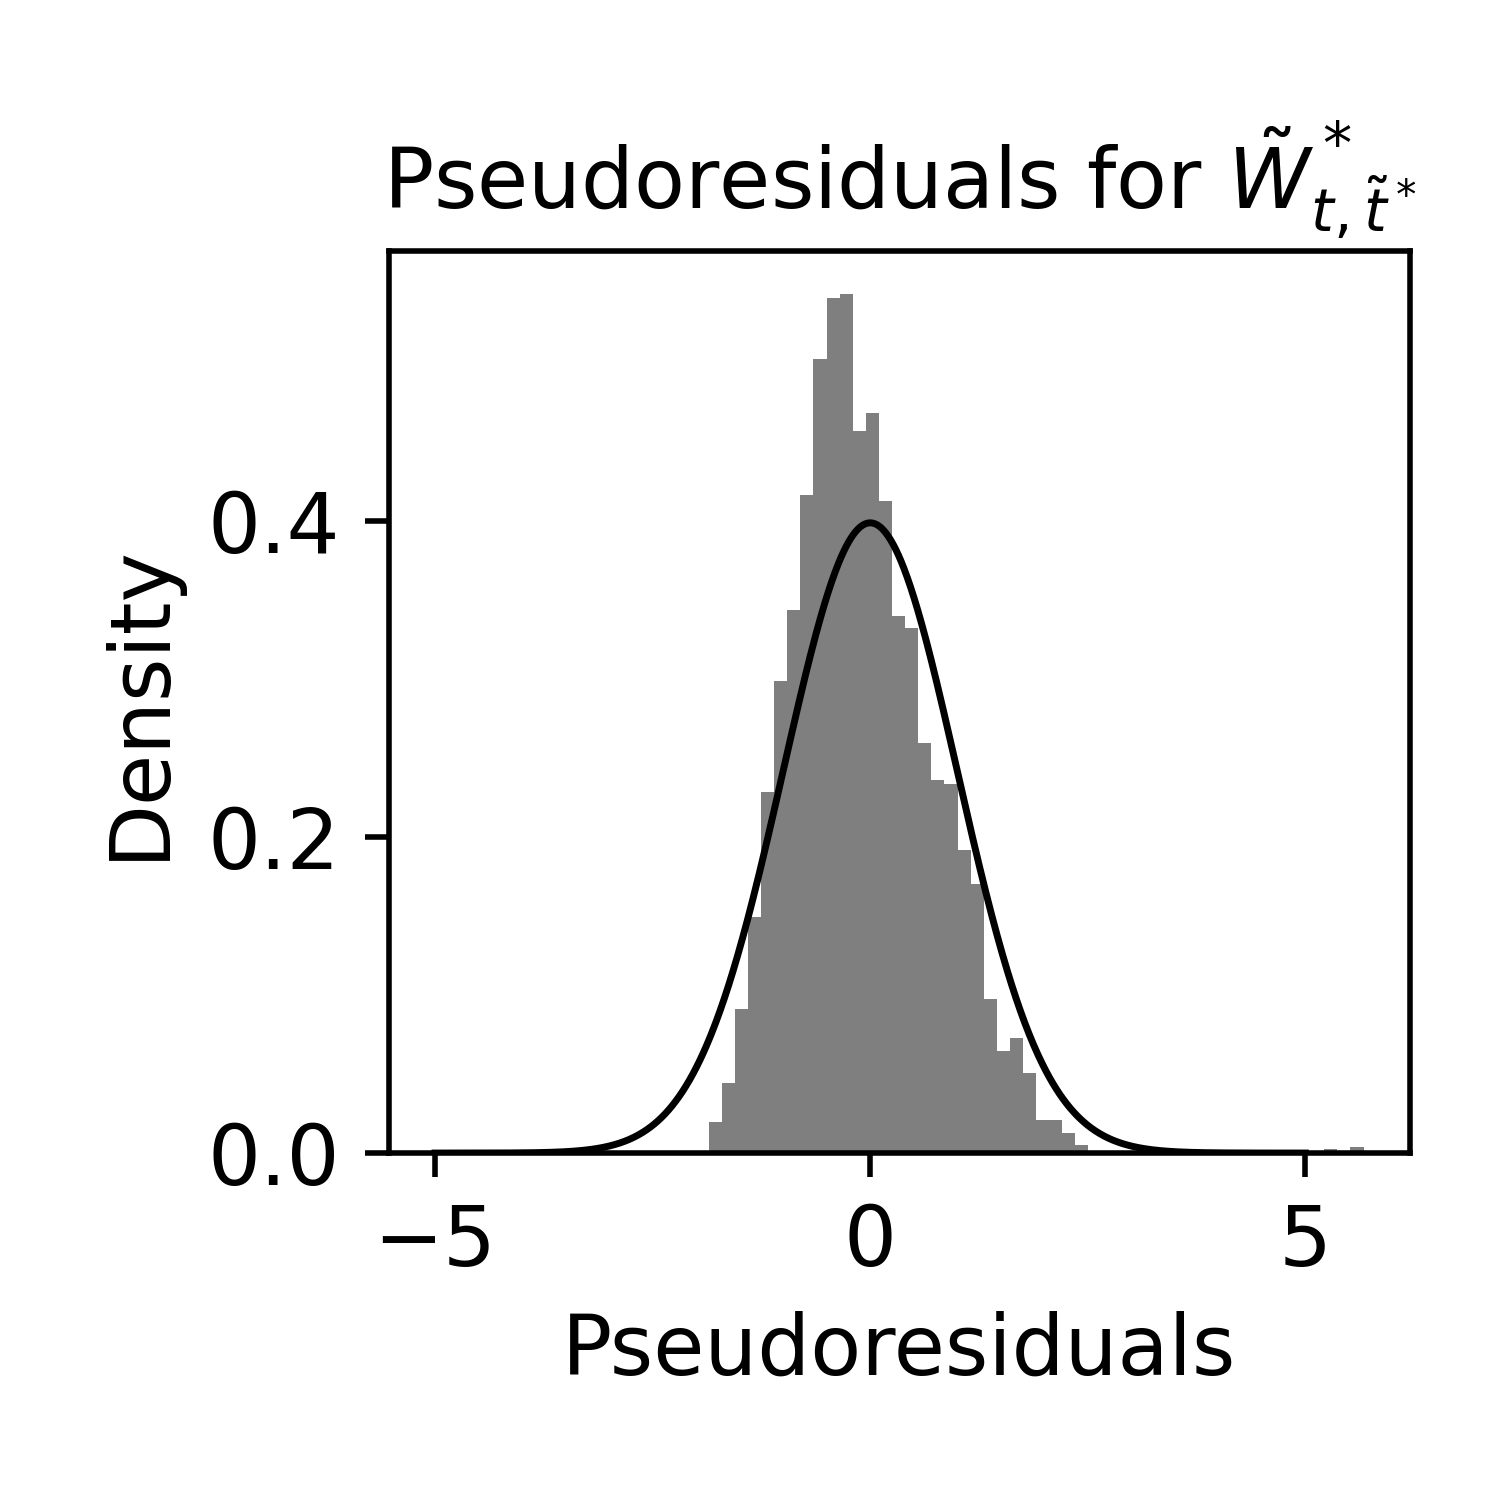
\includegraphics[width=2.25in]{../Plots/2019/20190902-182840-CATs_OB_1_0_267_CarHHMM2_pseudresids_ahat.png}
    	\caption{Histogram of pseudoresiduals of $\tilde W^*_{t,\tilde t^*}$}
    	\label{fig:pseudoresids}
    \end{subfigure}
    \begin{subfigure}{0.45\textwidth}
    	\centering
    	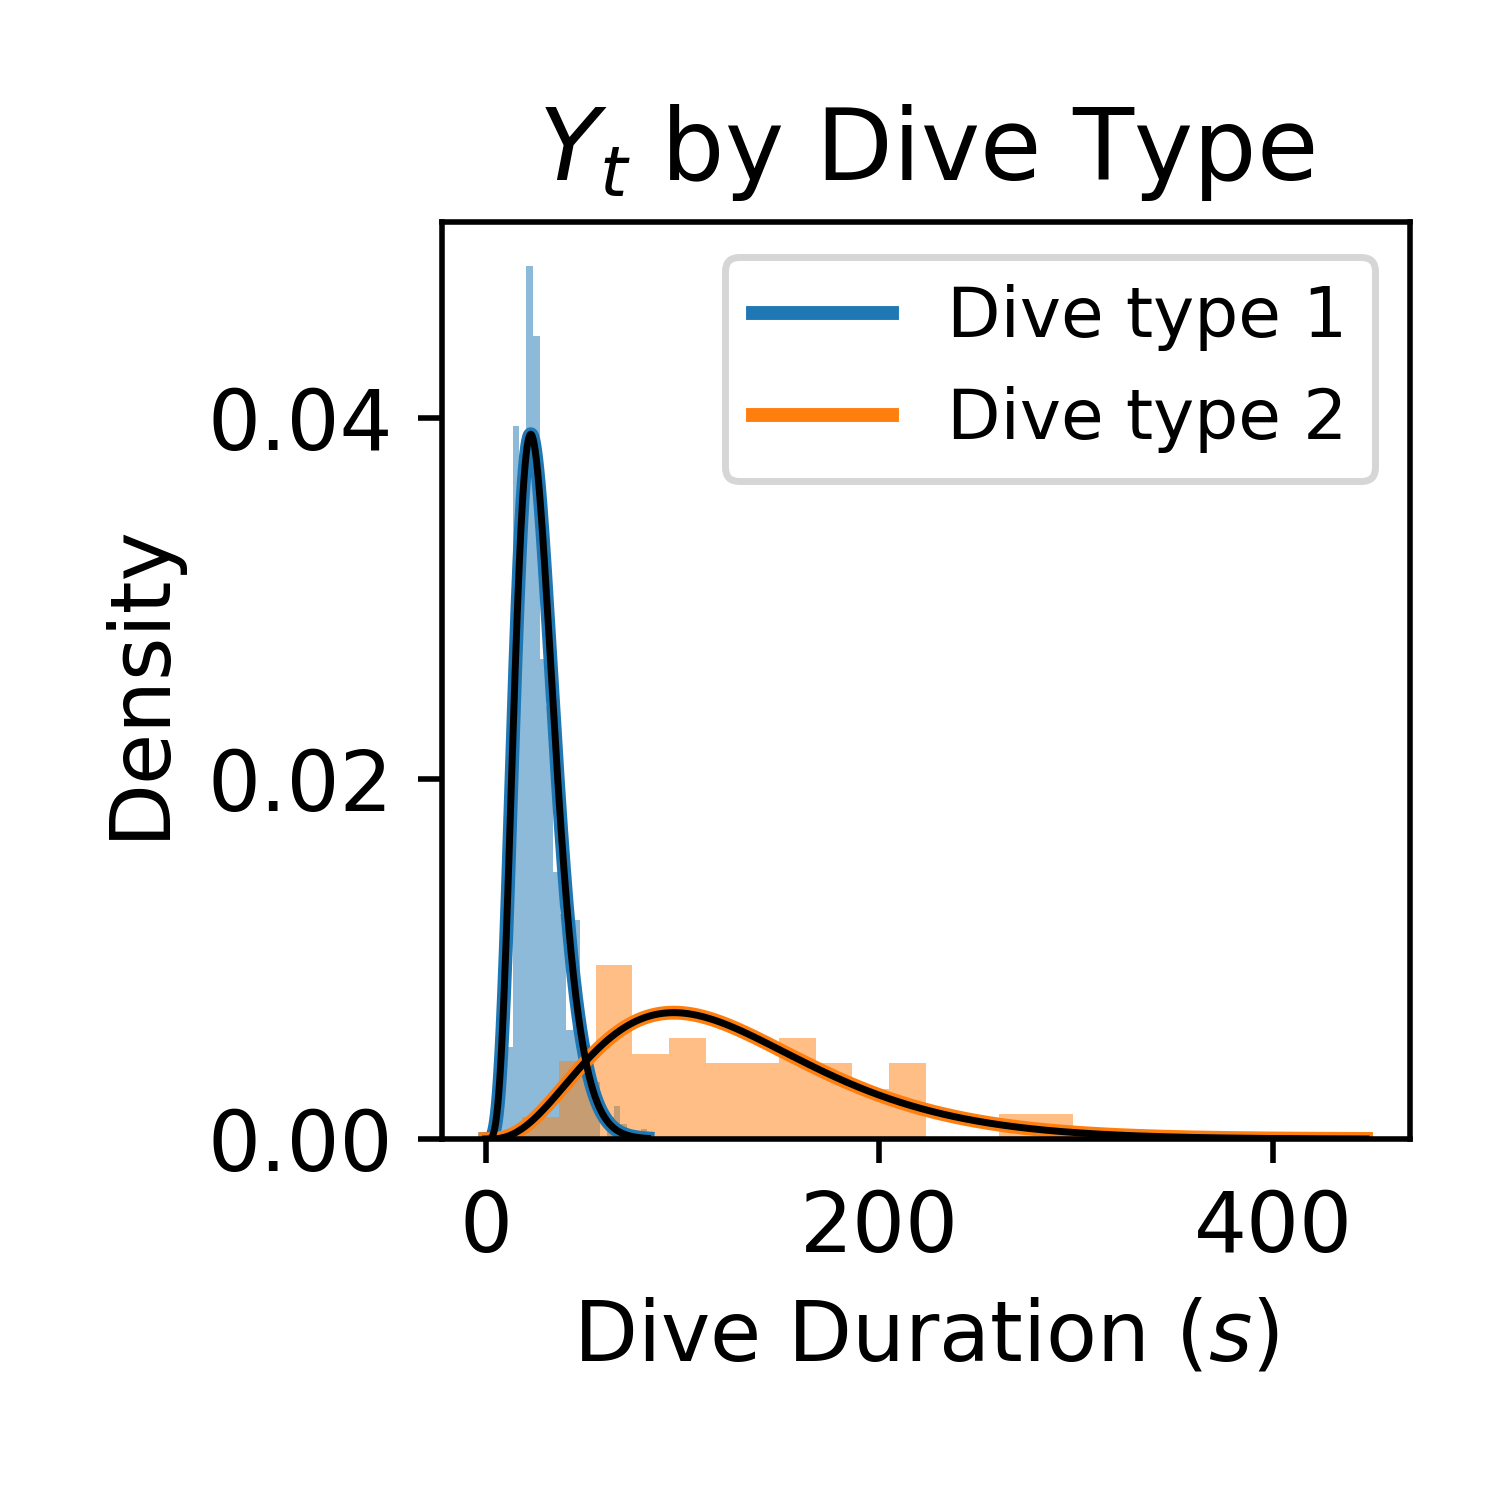
\includegraphics[width=2.25in]{../Plots/2019/20190902-182840-CATs_OB_1_0_267_CarHHMM2_empirical_hist_dive_duration.png}
    	\caption{Empirical distribution of $Y_t$}
    	\label{fig:empirical_dist}
    \end{subfigure}
    \caption{Pseudoresiduals of wiggliness 
    %$\left(\Phi^{-1} \left(\Pr(\Ztwo_{t,\tilde t^*} < \ztwo_{t,\tilde t^*}\big|Y,\tilde Y^* / \{\Ztwo_{t,\tilde t^*}\}) \right), \enspace \text{left} \right)$
    plotted over a standard normal density as well as a weighted empirical distribution of dive duration ($Y_t$, right) plotted over the corresponding fitted Gamma distributions. Both plots are generated by fitting the CarHHMM-DFT to the killer whale case study data and performing the forward-backward algorithm.}
    \label{fig:model_checking}
\end{figure}

%%% simulation study %%%

\begin{figure}[ht]
    \centering
    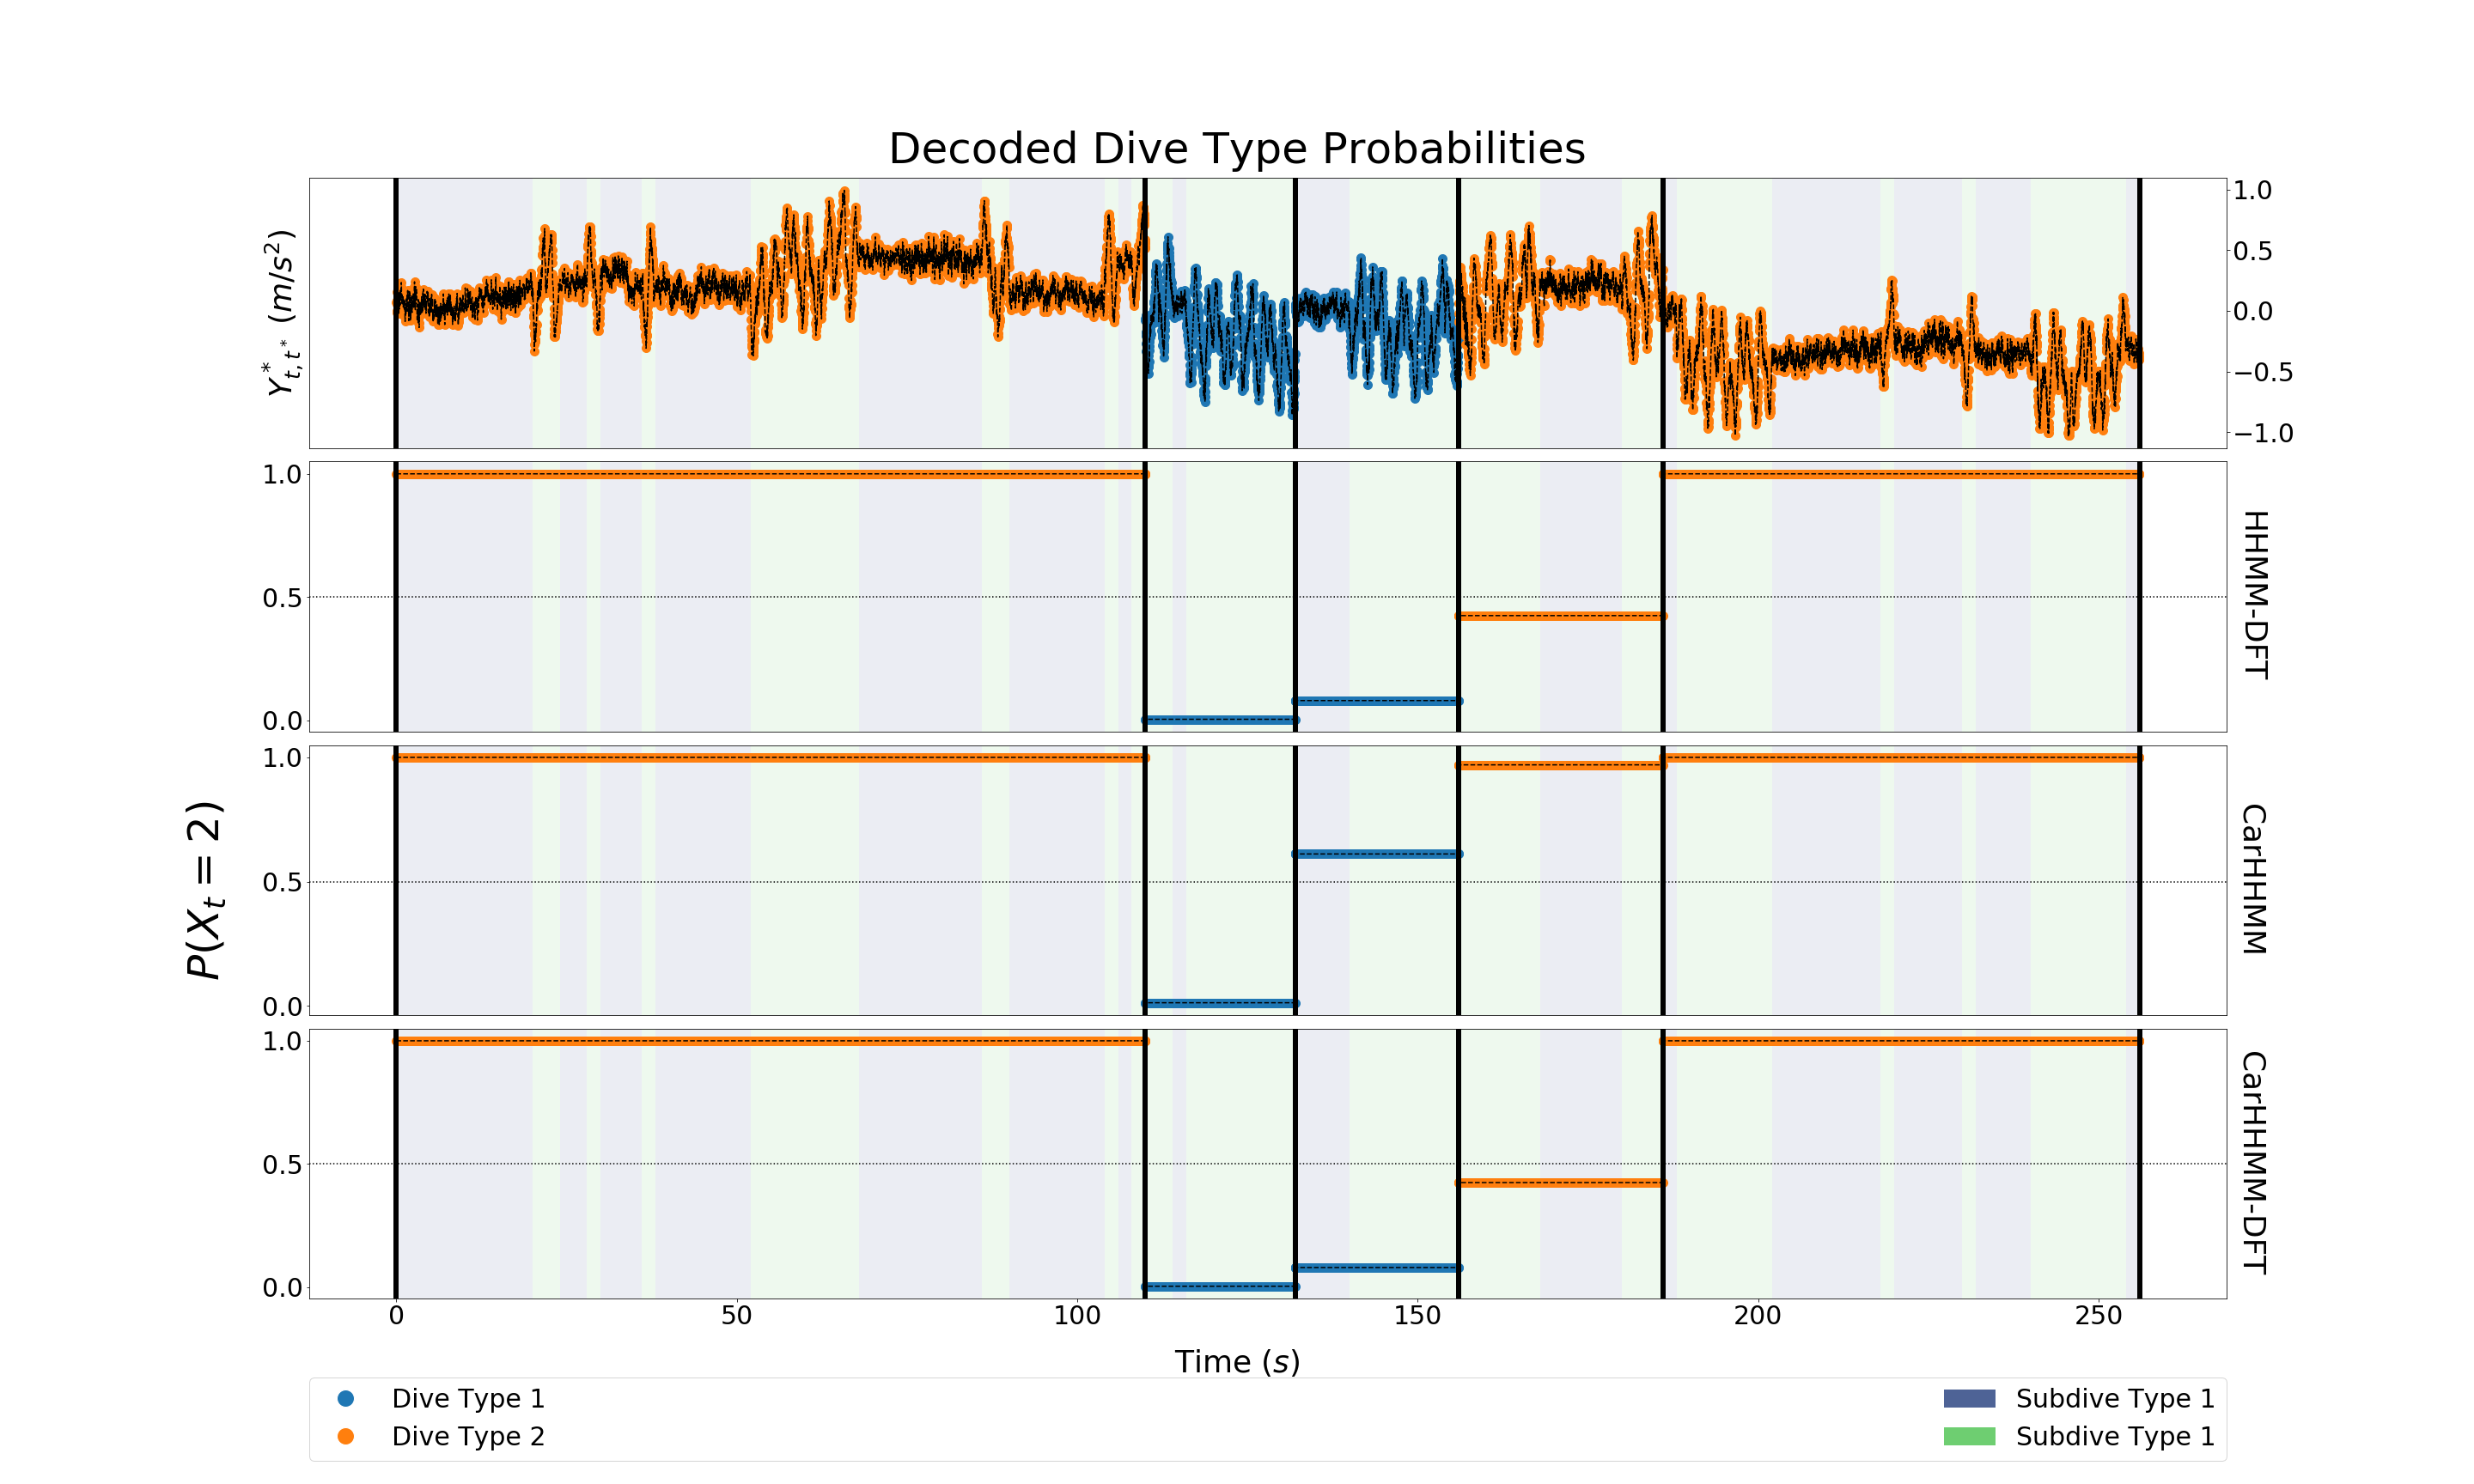
\includegraphics[width=4.5in]{../Plots/Posterior_Coarse_States.png}
    \caption{Estimated probabilities that each dive is of type 2 for five selected dives of a simulated data set of killer whale dive behaviour. Each panel is partitioned into dives by vertical black lines. The colour of the curve corresponds to the true dive type while the colour of the background corresponds to the true subdive state. The CarHMM-DFT is omitted because it assumes that there is only one dive type.}
    \label{fig:acc_coarse}
\end{figure}

\begin{figure}[ht]
    \centering
    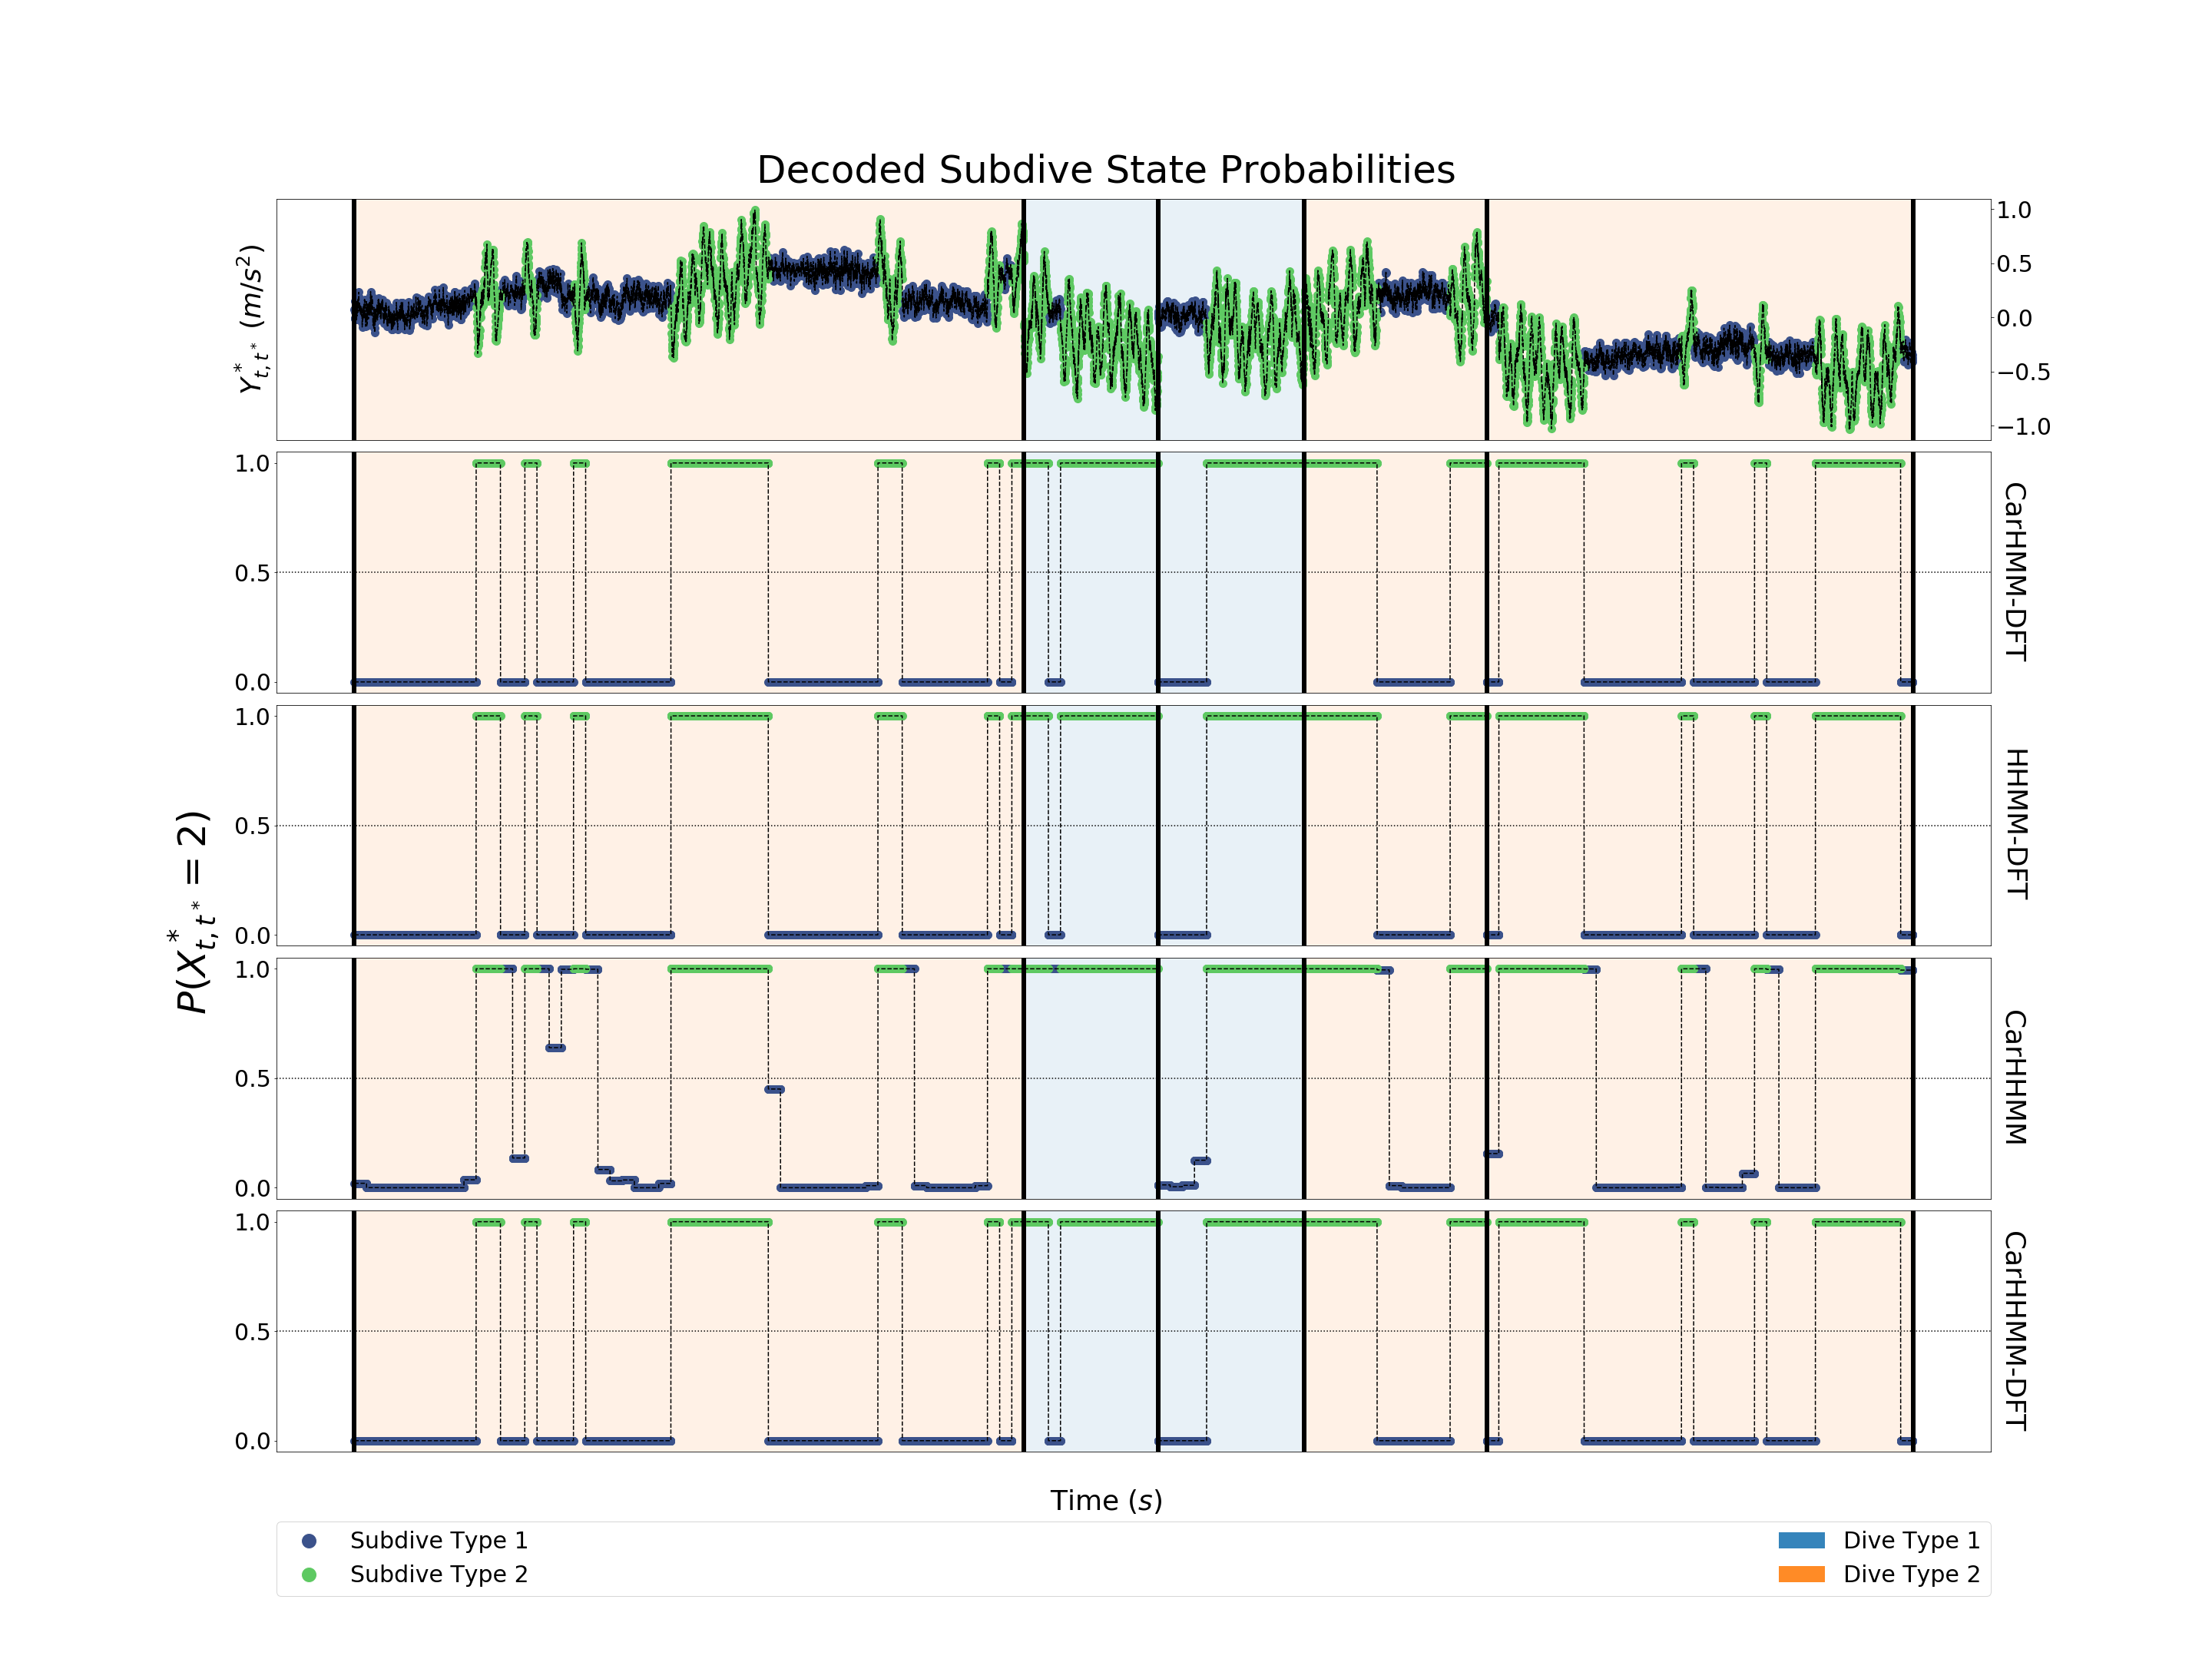
\includegraphics[width=4.5in]{../Plots/Posterior_Fine_States.png}
    \caption{Estimated probabilities that each window corresponds to subdive state 2 for five selected dives of a simulated data set of killer whale dive behaviour. Each panel is partitioned into dives by vertical black lines. The colour of the curve corresponds to the true subdive state while the colour of the background corresponds to the true dive type.}
    \label{fig:acc_fine}
\end{figure}